% Packages (fold)
\RequirePackage{lmodern}
\documentclass[12pt, oneside, extrafontsizes]{memoir}  % TODO 12pt, twoside

\setstocksize{11in}{8.5in}
\settrimmedsize{11in}{8.5in}{*}
\settrims{0in}{0in}
\setlrmarginsandblock{38mm}{25mm}{*}
\setulmarginsandblock{25mm}{25mm}{*}
\setheadfoot{13pt}{26pt}
\setheaderspaces{*}{13pt}{*}
\checkandfixthelayout
\DoubleSpacing
\setsecnumdepth{subsubsection}
\headstyles{default}
\chapterstyle{ell}
\setsecheadstyle{\scshape\LARGE\raggedright}

\usepackage[colorlinks,bookmarksnumbered,bookmarksdepth=subsubsection,unicode=true]{hyperref}
\newsubfloat{figure}  % must follow hyperref
\hypersetup{
pdfauthor = {Pierre Thodoroff},
pdftitle = {Temporal Regularization for Markov Decision Process},
pdfsubject = {Subject},
pdfkeywords = {reinforcement learning},
pdfcreator = {LaTeX with the hyperref package},
pdfproducer = {},
linkcolor = [HTML]{000000},
citecolor = [HTML]{0000FF},
}
\usepackage[utf8]{inputenc}
\usepackage{csquotes}
\usepackage{showidx}
\usepackage{amsmath}
\usepackage{amsfonts}
\usepackage{amssymb}
\usepackage{amsthm}
\usepackage{dsfont}
\usepackage{xspace}
\usepackage{tikz}
\usepackage{bbm}
\usetikzlibrary{shapes,arrows}
\usepackage{standalone}
\usepackage{amsmath,algorithmic,algorithm,setspace}


% Custom commands

\newtheorem{theorem}{Theorem}
\newtheorem{assumption}{Assumption}
\newtheorem{definition}{Definition}
\newtheorem{proposition}{proposition}
\newtheorem{lemma}{Lemma}
\newtheorem{corollaries}{Corollary}
\newtheorem{property}{Property}
\newtheorem*{remark}{Remark}
\usetikzlibrary{shapes,arrows}
\usepackage{standalone}
\newcommand{\param}{\beta}
\newcommand{\s}{\mathcal{S}}
\newcommand{\p}{\mathcal{P}}
\newcommand{\pol}{\pi}
\newcommand{\A}{\mathcal{A}}
\newcommand{\R}{\mathbb{R}}
\newcommand{\T}{\mathcal{T}}
\newcommand{\Q}{Q}
\newcommand{\Vr}{\V_{\param}}
\newcommand{\V}{V}
\newcommand{\regT}{\T^{\pol}_{\param}}
\newcommand{\regTo}{\T^{*}_{\param}}
\newcommand{\expect}{\mathop{\mathbb{E}}}
\newcommand{\RE}{r}
\newcommand{\norm}[1]{\left\lVert#1\right\rVert}
\newcommand{\dr}{\widetilde{\delta}}
\newcommand{\qr}{\widetilde{Q}}
\newcommand{\pit}{\widetilde{\pi}}
\newcommand{\vr}{V^{\param}_{\theta}}
\newcommand{\vrb}{V^{\param}_{\theta,\omega}}
\newcommand{\Vt}{V_{\theta}}
\newcommand{\Vb}{V_{\theta,\omega}}

\newcommand{\Vm}{V_{\text{max}}}
\newcommand{\Rm}{R_{\text{max}}}
\newcommand{\Tvan}{\T^{\infty}_{\param}}
\makeindex

\usepackage[backend=biber, citestyle=authoryear, bibstyle=authoryear, isbn=false, url=false, doi=false, eprint=false, natbib=false, sorting=nty, uniquename=init]{biblatex}
\addbibresource{library.bib}

\begin{document}

%%%%%%%%%%%%%%%%%%%%%%%%%%%%%%%%%%%%%%%%%%%%%%%%%%%%%
% Title page
%%%%%%%%%%%%%%%%%%%%%%%%%%%%%%%%%%%%%%%%%%%%%%%%%%%%%

% Title (fold)
\pretitle{\begin{center}\cftchapterfont\huge}
\posttitle{\end{center}}
\preauthor{\begin{center}\huge}
\postauthor{\end{center}}
\predate{\begin{center}\large}
\postdate{\end{center}}

\title{Temporal Regularization for Markov Decision Process }
\author{Pierre Thodoroff}
\date{\today}
\renewcommand\maketitlehookb{
\vfill
}
\renewcommand\maketitlehookc{
\vfill
\begin{center}
{
\large
Computer Science\\
McGill University, Montreal
}
\end{center}
\vspace{10mm}
}
\renewcommand\maketitlehookd{
\vspace{10mm}
A thesis submitted to McGill University in partial fulfilment of the requirements of
the degree of Master of Science.
\copyright Pierre Thodoroff; \today.
}
% Title (end)

\begin{titlingpage}
\maketitle
\end{titlingpage}

%%%%%%%%%%%%%%%%%%%%%%%%%%%%%%%%%%%%%%%%%%%%%%%%%%%%%
% Ackowledgements
%%%%%%%%%%%%%%%%%%%%%%%%%%%%%%%%%%%%%%%%%%%%%%%%%%%%%
%\clearpage
%\pagenumbering{roman}
%\renewcommand{\abstractname}{Dedication}

%%%%%%%%%%%%%%%%%%%%%%%%%%%%%%%%%%%%%%%%%%%%%%%%%%%%%
% Ackowledgements
%%%%%%%%%%%%%%%%%%%%%%%%%%%%%%%%%%%%%%%%%%%%%%%%%%%%%
\clearpage
\pagenumbering{roman}
\renewcommand{\abstractname}{Acknowledgements}
\begin{abstract}
TODO
\end{abstract}

%%%%%%%%%%%%%%%%%%%%%%%%%%%%%%%%%%%%%%%%%%%%%%%%%%%%%
% Abstract
%%%%%%%%%%%%%%%%%%%%%%%%%%%%%%%%%%%%%%%%%%%%%%%%%%%%%
\clearpage
\renewcommand{\abstractname}{Abstract}
\begin{abstract}
Several applications of Reinforcement Learning suffer from instability due to high variance. This is especially prevalent in high dimensional domains. Regularization is a commonly used technique in machine learning to reduce variance, at the cost of introducing some bias. Most existing regularization techniques focus on spatial (perceptual) regularization.  Yet in reinforcement learning, due to the nature of the Bellman equation, there is an opportunity to also exploit temporal regularization based on smoothness in value estimates over trajectories.  In this thesis, we explore two methods to regularize value function estimates temporally. We first propose to exponentially smooth the target of TD methods using previous value estimates. We formally characterize the bias induced by this technique using Markov chain concepts. We illustrate the various characteristics via a sequence of simple discrete and continuous MDPs, and show that the technique provides improvement even in high-dimensional Atari games. The second method introduce    Recurrent Learning named from it's inspiration from Recurrent Neural Network. In this method, the value estimate of a state is exponentially smoothed with previous estimates along the trajectory.  We establish its asymptotic convergence properties under some smoothness assumption on the reward.  The proposed algorithm yields a natural way to learn a state dependent emphasis function that selectively learns to emphasize or ignore states based on trajectory information. We demonstrate the potential for this selective updating on a partially observable domain and several continuous control tasks.
\end{abstract}

%%%%%%%%%%%%%%%%%%%%%%%%%%%%%%%%%%%%%%%%%%%%%%%%%%%%%
% Abrégé
%%%%%%%%%%%%%%%%%%%%%%%%%%%%%%%%%%%%%%%%%%%%%%%%%%%%%
\clearpage
\renewcommand{\abstractname}{Résumé}
\begin{abstract}
Several applications of Reinforcement Learning suffer from instability due to high variance. This is especially prevalent in high dimensional domains. Regularization is a commonly used technique in machine learning to reduce variance, at the cost of introducing some bias. Most existing regularization techniques focus on spatial (perceptual) regularization.  Yet in reinforcement learning, due to the nature of the Bellman equation, there is an opportunity to also exploit temporal regularization based on smoothness in value estimates over trajectories.  In this thesis, we explore two methods to regularize value function estimates temporally. We first propose to exponentially smooth the target of TD methods using previous value estimates. We formally characterize the bias induced by this technique using Markov chain concepts. We illustrate the various characteristics via a sequence of simple discrete and continuous MDPs, and show that the technique provides improvement even in high-dimensional Atari games. The second method introduce    Recurrent Learning named from it's inspiration from Recurrent Neural Network. In this method, the value estimate of a state is exponentially smoothed with previous estimates along the trajectory.  We establish its asymptotic convergence properties under some smoothness assumption on the reward.  The proposed algorithm yields a natural way to learn a state dependent emphasis function that selectively learns to emphasize or ignore states based on trajectory information. We demonstrate the potential for this selective updating on a partially observable domain and several continuous control tasks.
\end{abstract}

%%%%%%%%%%%%%%%%%%%%%%%%%%%%%%%%%%%%%%%%%%%%%%%%%%%%%
% Table of content
%%%%%%%%%%%%%%%%%%%%%%%%%%%%%%%%%%%%%%%%%%%%%%%%%%%%%
\clearpage
\setcounter{tocdepth}{2}
\tableofcontents
%\newpage
%\listoffigures
%\listofalgorithms

%%%%%%%%%%%%%%%%%%%%%%%%%%%%%%%%%%%%%%%%%%%%%%%%%%%%%
% Introduction
%%%%%%%%%%%%%%%%%%%%%%%%%%%%%%%%%%%%%%%%%%%%%%%%%%%%%
\clearpage
\pagenumbering{arabic}
\chapter{Introduction}
% TODO write the intro

Reinforcement Learning is a mathematical framework designed to model sequential decision making. It is used to solve a wide range of control tasks ranging from video games \cite{vinyals2017starcraft,mnih2013playing,mnih2016asynchronous} to robotics \cite{kober2013reinforcement,abbeel2010autonomous}. It is also used in many real-life applications such as hydro control \cite{grinberg2014optimizing} and power grid management \cite{franccois2016deep}.


There has been much progress in Reinforcement Learning (RL) techniques, with some impressive success with games \cite{silver16}, and several interesting applications on the horizon \cite{koedinger18,shortreed11,prasad17,dhingra17}. In this thesis we focus on value based reinforcement learning. 
INTRO VALUE BASED ..
However RL methods are too often hampered by high variance, whether due to randomness in data collection, effects of initial conditions, complexity of learner function class, hyper-parameter configuration, or sparsity of the reward signal \cite{henderson2017deep}.
We propose 2 method to mitigate those issue
Regularization is a commonly used technique in machine learning to reduce variance, at the cost of introducing some (smaller) bias.  Regularization typically takes the form of smoothing over the observation space to reduce the complexity of the learner's hypothesis class.

In the RL setting, we have an interesting opportunity to consider an alternative form of regularization, namely temporal regularization.  Effectively, temporal regularization considers smoothing over the trajectory, whereby the estimate of the value function at one state is assumed to be related to the value function at the state(s) that typically occur before it in trajectories. This structure arises naturally out of the fact that the value at each state is estimated using the Bellman equation. The standard Bellman equation clearly defines the dependency between value estimates. In temporal regularization we amplify this dependency by making each state depend more strongly on estimates of \emph{previous} states as opposed to multi-step that considers future states. 

This paper proposes a class of temporally regularized value function estimates. We discuss properties of these estimates, based on notions from Markov chains, under the policy evaluation setting and extend the notion to the control case.
Our experiments show that temporal regularization effectively reduces variance and estimation error in discrete and continuous MDPs.  The experiments also highlight that regularizing in the time domain rather than in the spatial domain allows more robustness to cases where state features are mis-specified or noisy, as is the case in the Atari domains.


\section{Intro part 2}
Graph smooth estimate like time series
\begin{itemize}
    \item Fitting a model
    \item averaging of previous values
    \item Entropy term 
\end{itemize}


\section{Introduction}

Reinforcement learning algorithms often suffers from variance issues. In particular, we describe two issues that Recurrent Learning attempts to mitigate. The first one considers the \emph{variance of the value estimates through the trajectory}. Consider a hypothetical scenario in which a person is driving a car at a high speed. Its behavior needs to be temporally coherent. If the driver wants to change lane, there needs to be a continuous smooth decision making process. For the policy of the driver to be coherent, its value function needs to be temporally smooth. Most algorithms make a decision at every time step without necessarily \emph{explicitly} enforcing temporal coherence nor considering previous decisions. This can lead to erratic and temporally inconsistent behaviors, particularly in tabular and discrete settings. The second issue considers the limited capacity of the brain to process information and make decision. Bounded rationality argues that human brain has a limited capacity to learn and can't store all the information. In this work we argue that the capacity to ignore or emphasize chosen state is a key component for the success of decision making algorithms.  

%%%%%%%%%%%%%%%%%%%%%%%%%%%%%%%%%%%%%%%%%%%%%%%%%%%%%
% Background
%%%%%%%%%%%%%%%%%%%%%%%%%%%%%%%%%%%%%%%%%%%%%%%%%%%%%
\chapter{Markov Chains}
\label{chap:markov}
\section{Discrete-time Markov chains}
We begin by introducing discrete Markov chain concepts that will be used to study the properties of temporally regularized MDPs. In this thesis, we focus on discrete Markov chains, however the concepts can be extended to the continuous case.\\ Discrete Markov chain are stochastic models representing sequences of random variable satisfying the Markov property. Formally, we define a discrete-time Markov chain (\cite{norris1998markov,levin2017markov,bremaud2013markov})  with finite state space $\s$ by a sequence of $|\s|-$valued random variable $X_0,X_1,..$. and a transition function $\p : \s \times \s \mapsto [0,1]$. The sequence of random variable needs to satisfy the Markov property:
\begin{definition}
A stochastic process satisfy Markov property if:
\begin{equation}
    \p (X_{n+1}=j|X_n = i,X_{n-1}=k,...) = \p (X_{n+1}=j|X_n = i)
\end{equation}
\end{definition}
Intuitively, this means that the probability of moving to the next states is based solely on its present state and not its history. One of the most studied Markov chains considers the property of randomly walking on a chain as described in figure (\ref{fig:random_walk}).\\
\begin{figure}
    \centering
    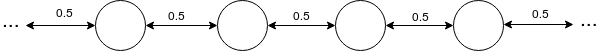
\includegraphics[scale=0.7]{fig/Markov_chain.png}
    \caption{Random walk}
    \label{fig:random_walk}
\end{figure}
Discrete time Markov chains can also be represented in matrix form. The transition function can be represented as a $|\s| \times |\s|$ matrix P such that $P_{ij} = \p(X_{n+1}=j|X_n=i)$. Studying Markov chains from an algebraic perspective can sometimes simplify the analysis.  \\
We now define some useful fundamental properties of Markov chains.
If every state is accessible from every other, the chain(or its transition matrix) is said to be irreducible. 
\begin{definition}
A chain is said to be irreducible if $\forall i,j \in \s$ there exists $n \in \mathbb{N}$ such that:
\begin{equation}
      \quad P(X_n = j|X_0=i) > 0
\end{equation}
\end{definition}
\begin{definition}
The period of a state is the greatest common divisor of the set {$n \in  \mathbb{N} : \quad P(X_n=i|X_0=i) > 0$}. The chain is defined as aperiodic if every state has period 1.
\end{definition}
\begin{definition}
Let $T_i$ define the hitting time of state i such that:
\begin{equation}
    T_i = inf(n \geq 1 : X_n = i | X_0 = i)
\end{equation}
We define a transient state if $T_i$ is not finite. A state is called recurrent if it is not transient.
\end{definition}
\begin{definition}
A chain is defined as ergodic if it is positive recurrent and aperiodic.
\end{definition}
Throughout this thesis, we make the following mild assumption on the Markov chain:
\begin{assumption}
P is ergodic
\end{assumption}
Most of the Reinforcement learning theory relies on this assumption. However, some works considers the case when the chain is not ergodic (\cite{leike2016nonparametric}).

\section{Stationary distribution}
It is often interesting to study the properties of Markov chains in the limit. We define the stationary distribution $\mu_i$ as the \emph{proportion of time} spend in each state $i \in \s$.
\begin{definition}
Assuming that P is ergodic, P has a unique stationary distribution $\mu$ that satisfies:
\begin{equation}
\begin{split}
    \mu &= \mu P \\
    \sum_i \mu_i &= 1
\end{split}
\end{equation}
\end{definition}
There exists many different metrics used to define distance's from stationary distribution (\cite{levin2017markov}). One common metric in discrete Markov chains can be defined as follows:
\begin{equation}
    d_t(P) = \norm{P^t \mathbbm{1} - \mu}_{ \infty } 
    \label{eq:d_markov}
\end{equation}
where $\mathbbm{1}$ is a vector of one's.
\section{Detailed Balance}
The concept of detailed balance originated from physics. It is used to study the behavior of systems in the limit at \emph{equilibrium}. 
\begin{definition}[Detailed balance~\cite{kemeny1976finite}]
Let $P$ be an irreducible Markov chain with invariant stationary distribution $\mu$. $\mu_i$ defines the $i$th element of $\mu$. A chain is said to satisfy detailed balance if and only if
\begin{equation}
    \mu_i P_{ij} = \mu_j P_{ji} \qquad \forall i,j \in \s.
\end{equation}
\end{definition}
Intuitively, this means that if we start the chain in a stationary distribution, the amount of probability that flows from $i$ to $j$ is equal to the one from $j$ to $i$. In other words, the system must be at equilibrium. An intuitive example of a physical system not satisfying detailed balance is a snow flake in a coffee. 
\begin{remark}
If a chain satisfies detailed balance, it is called reversible.
\end{remark}

\section{Mixing Time}

In Markov chains theory, one of the main challenges is to study the mixing time of the chain (\cite{levin2017markov}). The mixing time corresponds to the time needed for the chain to be \emph{close} to its stationary distribution $\mu$. More formally it can be defined as:
\begin{equation}
    t_{mix}(\epsilon) = \text{min} \{ t : d_t(P) < \epsilon \}
\end{equation}
where $d_t(P)$ can be defined as in (\ref{eq:d_markov}).\\
When the chain is reversible, it is possible to estimate and bound the mixing time relatively efficiently (\cite{diaconis1991geometric,}). Indeed, many chains do not satisfy this detailed balance property. In this one case it is possible to use a different, but related, chain called the reversal Markov chain to infer mixing time bounds (\cite{fill1991eigenvalue,chung2012chernoff}).




\section{Reversal Markov Chains}
The reversal Markov chain $\widetilde{P}$ can be interpreted as the Markov chain $P$ with time running backwards. It is be a key concept used to define convergence and bias induced by temporal regularization later in this thesis. 
\begin{definition}[Reversal Markov chain~\cite{kemeny1976finite}]
Let $\widetilde{P}$ the reversal Markov chain of $P$ be defined as:
\begin{equation}
    \widetilde{P_{ij}} = \frac{\mu_j P_{ji}}{\mu_i} \qquad \forall i,j \in \s.
\end{equation}
\end{definition}
As an example, assuming a Markov chain P has a uniform stationary distribution, if a transition is highly irreversible like falling off a cliff ($P_{ij} \# P_{ji}$) the difference between the forward and the backward chain in that state will be high. We now introduce some properties of reversal Markov chains that will be used later in the thesis.
\begin{remark}
If $P$ is irreducible with invariant distribution $\mu$, then $\widetilde{P}$ is also irreducible with invariant distribution $\mu$.
\end{remark}

\begin{remark}
If $P$ is reversible than $P = \widetilde{P}$
\end{remark}
Furthermore, both $P$ and $\widetilde{P}$ have the same stationary distribution and so does any convex combination of them.

\begin{lemma}
$P$ and $(1-\param) P + \param \widetilde{P}$ have the same stationary distribution $\mu \quad \forall \param \in [0,1]$.
\end{lemma}
\begin{proof}
\begin{equation}
    \begin{split}
        \mu ( (1-\param) P + \param \widetilde{P}) &=  (1-\param) \mu P + \param \mu \widetilde{P} \\
        &= (1-\param)\mu + \param \mu\\
        &= \mu.
    \end{split}
\end{equation}
\end{proof}




\chapter{Reinforcement Learning}
\label{chap:reinforcement}
In science, mathematical frameworks are used to study the behavior of objects. In physics, for example, the newton's laws laid the foundation of classical mechanics used to describe the motion of macroscopic objects.
In this thesis, we are interested in the problem of sequential decision making. The most popular mathematical framework used to study sequential decision making is called Markov Decision Process(MDP). The underlying core assumption is the Markovian assumption on the state space. MDP assumes the state space is fully observable and the future is independant of the past conditioned on the current state. More formally, this can be described as:
\begin{equation}
        p(s_{t+1} | s_{t},s_{t-1},...,s_0) = p(s_{t+1} | s_t)
\end{equation}
Sequential decision making differs from supervised learning in several ways. Supervised learning is a set of models designed to predict an output based on IID data. However, in reinforcement learning our prediction/decision often impact the distribution of the data. For example, choosing to do turn right at an intersection will siginificantly change the distribution of future states. 

\section{Markov Decision Process}
We now formally introduce the concept used in Markov Decision Process.
\begin{definition}[Markov Decision Process ~(\citep{puterman2014markov})]
A Markov Decision Process (MDP) is defined as a tuple ($\s,\p,\RE$) where:
\begin{itemize}
    \item $\s$ is a discrete set of states 
    \item $\p : \s \times \A \times \s \mapsto [0,1]$ is a transition function 
    \item  $\RE : \s \times \A \mapsto \R$ is a reward function
\end{itemize}
\end{definition}
On each round $t$, the learner observes current state $s_t\in\s$ and selects action $a_t\in\A$, after which it receives reward $r_t = \RE(s_t,a_t)$ and moves to new state $s_{t+1}\sim \p(\cdot|s_t, a_t)$. We define a stationary policy $\pol$ as a probability distribution over actions conditioned on states $\pol : \s \times \A \mapsto [0,1]$, such that $a_t \sim \pol(\cdot|s_t)$.

\section{Policy Evaluation}
For policy evaluation,  given a policy $\pol$, the goal is to find the associated value function of that policy $v^{\pol}$. 
When performing policy evaluation in the discounted case, the goal is to estimate the discounted expected return of policy $\pol$ at a state $s\in\s$,  $\V^{\pol}(s) = \expect_{\pol}[\sum_{t=0}^{\infty} \gamma^t \RE_{t+1} | s_0 = s]$, with discount factor $\gamma \in [0,1)$. This can be written in matrix form as:
\begin{equation}
     v^{\pol} = \sum_{i=0}^{\infty} \gamma^i (P^{\pol})^i r
\end{equation}
where $P^{\pol}$ denotes the $|\s|\times |\s|$ transition matrix under policy $\pol$, $v^\pi$ is the state values column-vector, and $r$ is the reward column-vector. The actions do not appear in the equations explicitly as the policy has been coupled inside $P^{\pol}$.The matrix $P^{\pol}$ also defines a Markov chain.
In practice, we often do not have  access to the transitions and rewards directly. Instead, we sample tuples $(s,s',r)$ from the environment and use those to estimate in expectation the discounted expected cumulative return for a state.
The most straightforwad way to estimate $v$ would be to collect tuples $(s,s',r)$  and average the discounted reward. However, this often suffers from high variance (\citep{kearns2000bias}). By unrolling the discounted sum of reward it is possible to obtain a recursive form based on $v$:
\begin{equation}
\label{equ:bellman}
\begin{split}
    v^{\pol}(s_0) &=  \expect_{\pol}[\RE (s_0,\pol(s_0)) + \sum_{t=1}^{\infty} \gamma^t \RE_{t+1} | s_0 = s] \\
    &=  \expect_{\pol}[\RE (s_0,\pol(s_0)) + \gamma \expect_{\pol}[\sum_{t=0}^{\infty} \gamma^t \RE_{t+1}|s_1] | s_0 = s]\\
    &= \expect_{\pol}[\RE (s_0,\pol(s_0)) + \gamma v^{\pol}(s_1) | s_0 = s] \\
\end{split}
\end{equation}
This can also be rewritten as a linear system of equation and solved using standard algebra methods:
\begin{equation}
\label{eq:fixed_point}
\begin{split}
    & v^{\pol} = r + \gamma P^{\pol}v^{\pol} \\
    &\equiv (I-P^{\pol})v^{\pol} = r
\end{split}
\end{equation}
However, inverting a matrix can be costly, unstable and as mentioned earlier in practice we often do not have access to $P^{\pol},r$ directly. This suggests that using iterative method may be more suitable for reinforcement learning.
\subsection{Bellman Operator}
We consider the operator-theoretic point of view by defining the following operator
\begin{definition}
The Bellman operator $\T^{\pol}$ has a unique fixed point $v^{\pol}$  where:
\begin{equation}
\label{equ:bell_pol}
   \T^{\pol} v = r + \gamma P^{\pol} v
\end{equation}
\end{definition}
In order to show this we use Banach Fixed point theorem stating that:
\begin{theorem}[Banach Fixed Point Theorem (\citep{banach1922operations})]
Let U be a Banach space: if $\T U \rightarrow U$ is a contraction mapping then:
\begin{itemize}
    \item There exists a unique fixed point $v^*$ such that $\T v^* = v^*$
    \item $lim_{t \rightarrow \infty} \T^tv = v^*$ 
\end{itemize}
\end{theorem}

As we saw in the previous section in equation \ref{eq:fixed_point} $v^{\pol}$ is a fixed point. We can prove its unicity and the convergence of the operator by proving that $ \T^{\pol}$ is a contraction. In this thesis, unless stated otherwise, the norm considered is the infinity norm.
\begin{lemma}
$\T^{\pol}$ is a contraction with a contraction factor of $\gamma$
\end{lemma}
\begin{proof}
\begin{equation}
\begin{split}
    \norm{\T^{\pol}u - \T^{\pol} v} &= \norm{r+\gamma P^{\pol}u - (r + \gamma P^{\pol} v} \\
    &= \norm{\gamma P^{\pol}(u - v)}\\
    &= \gamma \norm{u-v}
\end{split}
\end{equation}
\end{proof}
Algorithm \ref{alg:pol_eval} shows an example of a stochastic version of equation \ref{equ:bell_pol}.\\

\begin{algorithm}[H]
\caption{Policy evaluation}
\begin{algorithmic}[1]
    \STATE Input: $\pi,\gamma$
    \FORALL{steps}
        \STATE Choose $a \sim \pi(\s)$
        \STATE Take action $a$, observe $r(s),s'$
        \STATE $\V(s) =  r(s) + \gamma \V(s') $
    \ENDFOR
\end{algorithmic}
\label{alg:pol_eval}
\end{algorithm}
It is also possible to study the stochastic version of this operator using techniques from dynamical system and ordinary differential equations (\citep{borkar2000ode}).


\subsection{Temporal Difference}
At each step of the bellman operator the previous estimate $v^{\pol}_t$ at time step t is forgotten.
\begin{equation}
    v_{t+1} = r + \gamma P v_{t}
\end{equation}
Temporal difference attempts to exploit previous estimates by averaging them such that $v_{t+1} = \alpha \sum_{i=0}^{t+1} (1-\alpha)^{t-i} v_i$
\begin{equation}
\begin{split}
    v_{t+1} &= \alpha  (r + \gamma P v_{t}) + (1-\alpha) v_{t} \\
    &= \alpha  (r + \gamma P v_{t}) + (1-\alpha) [\alpha (r + \gamma P v_{t-1}) + (1-\alpha) v_{t-1}]
\end{split}
\end{equation}
This gives rise to the temporal difference algorithm:
\begin{equation}
\begin{split}
    v_{t+1} &= \alpha  (r + \gamma P v_{t}) + (1-\alpha) v_{t} \\
    &= \alpha (r + \gamma P v_{t} - v_{t}) + v_{t}
\end{split}
\end{equation}
\begin{definition}[Temporal Difference ~(\citep{sutton1988learning})]
The temporal difference operator $\T_{\alpha}$ parametrized by $\alpha$ can be written as:
\begin{equation}
\begin{split}
    \T_{\alpha} v &= (1-\alpha)v + \alpha(r + \gamma Pv) \\
\end{split}
\end{equation}
\end{definition}

A stochastic version of temporal difference can be found in algorithm \ref{alg:temporal_difference}.\\
\begin{algorithm}[H]
\caption{Temporal Difference}
\begin{algorithmic}[1]
    \STATE Input: $\pi,\alpha,\gamma$
    \FORALL{steps}
        \STATE Choose $a \sim \pi(\s)$
        \STATE Take action $a$, observe $r(s),s'$
        \STATE $\V(s) = \V(s) + \alpha (r(s) + \gamma \V(s')-\V(s)) $
    \ENDFOR
\end{algorithmic}
\label{alg:temporal_difference}
\end{algorithm}


Bootstrapping on previous estimates may introduce bias depending on how well $v$ is estimated. Several papers attempt to characterize this bias in various ways (\citep{kearns2000bias,sutton1994step}). Methods bootstrapping on previous estimates are also called semi-iterative methods (\citep{varga2009matrix}) in the field of iterative methods. It would be interesting to examine algorithms like chebyshev semi-iterative method (\citep{golub1961chebyshev}) that attempts to find optimal $\alpha$'s using chebyshev polynomials. There might exists interesting connections with meta-learning algorithms.
\subsection{Lambda Return}
In the previous sections we defined algorithms that bootstrap on the next value, to reduce variance, instead of looking at the rewards. Lambda return (\citep{sutton1984temporal}) generalizes this intuition by bootstrapping on all future values, not just the direct next one. This is done by first unrolling the bellman updates, yielding N-step return of the form:
\begin{definition}[N-step return]
\begin{equation}
    \T_{n} = \sum_{i=0}^{n} \gamma^i r + \gamma^{n+1} Pv
\end{equation}
\end{definition}
Instead of choosing a specific N, lambda-return exponentially averages through all the N-step return.
\begin{definition}[Lambda-return]
\begin{equation}
    \T^{(\lambda)} = (1-\lambda) \sum_{i=0}^{\infty} \lambda^i \T_{i}
\end{equation}
\end{definition}

Varying $\lambda$ yields Monte Carlo on one side ($\lambda \rightarrow 1$) and TD(0) on the other ($\lambda \rightarrow 0$).
Lambda-return can be implemented efficiently in an online fashion using eligibility traces (\citep{sutton1984temporal,singh1996reinforcement,precup2000eligibility}).\\
\begin{algorithm}[H]
\caption{Temporal Difference with eligibility traces}
\begin{algorithmic}[1]
    \STATE Input: $\pi,\alpha,\gamma,\lambda$
    \FORALL{steps}
        \STATE Choose $a \sim \pi(\s)$
        \STATE Take action $a$, observe $r(s),s'$
        \STATE $e(t) =  \mathbb{1}_{s}+ \gamma \lambda e(t-1)$
        \STATE $\V = \V + \alpha (r(s) + \gamma \V(s')-\V(s)) e(t)$
    \ENDFOR
\end{algorithmic}
\label{alg:eligibility_traces}
\end{algorithm}
However, this algorithm is biased if the trace is used online. This is due to the fact that when an update is done, the trace becomes biased as the distribution with respect to the new parameters would have been different. True online TD (\citep{seijen2014true}) solves this issue by accounting for those changes. This problem is similar to the one encountered by real time recurrent learning (\citep{williams1995gradient}). It would be interesting to study if True Online TD can be extended to the non-linear settings. 
\subsection{Linear Function Approximation}
The methods developed previously scale linearly with the number of states. This becomes quickly intractable for large discrete state space and continuous settings. One way to remedy this is to use function approximation. It is possible to develop similar operators using function approximator.
The aim is to find a function $V_\theta: \mathbb{S} \rightarrow \mathbb{R}$ parametrized by $\theta$ that approximates $V^{\pol}$. We can fall back to the tabular setting by representing the states in a one hot vector form with $\theta \in \mathbb{R^{|\mathbb{S}|}}$. The goal is to find a set of parameters $\theta$ that minimizes the squared loss:
\begin{equation}\label{simple_loss}
    \mathcal{L}(\theta) = \expect_{\pol} [(V^{\pol} - V_\theta)^2]
\end{equation}
which yields the following update by taking the derivative with respect to $\theta$:
\begin{equation}
    \theta_{t+1} = \theta_t + \alpha (V^{\pol}(s_t) - V_{\theta_t}(s_t)) \nabla_{\theta_t} V_{\theta_t}(s_t)
\end{equation}
where $\alpha$ is a learning rate.\\
In practice $V^{\pol}$ is approximated using Monte Carlo rollouts (\citep{suttonreinforcement}) or TD methods (\citep{sutton1988learning}).

\subsection{Convergence using Stochastic Approximation}
Convergence in the stochastic setting is usually proven by casting the learning algorithm as a stochastic approximation (\citep{tsitsiklis1994asynchronous,borkar2009stochastic,borkar2000ode}) of the form:
\begin{equation}\label{stoch}
    \theta_{t+1} = \theta_t + \alpha( \T \theta_t  - \theta_t + w(t)) 
\end{equation}
where $\T: \mathbb{R^{|\mathbb{S}|}} \rightarrow \mathbb{R^{|\mathbb{S}|}}$ is a contraction operator and $w(t)$ is a noise term. 
As an example, TD(0) is known to converge to the fixed point of the bellman operator (\citep{sutton1988learning}):
\begin{equation}
    \T \Vt(s_t) = \expect_{s_{t+1} \sim \pol} [r(s_t) + \gamma \Vt(s_{t+1})]
\end{equation}
However, in practice we have access to a noisy version of the operator $\widetilde{\T}$ due to sampling process hence the noise term $w(t)$:
\begin{equation}
    w(t) = r_t + \gamma \Vt (s_{t+1}) - \expect_{s_{t+1} \sim \pol} [r + \gamma \Vt(s_{t+1})]
\end{equation}

\section{Control}
In the previous section we discussed estimating the value of a policy. However, in many cases, the actual goal is to use this estimate to \emph{improve} on the policy. This is called control.
\subsection{Bellman Optimilatiy Equations}
In the control case, the goal is to find the optimal policy $\pol^*$ that maximizes the discounted expected return. As in the previous section we define the optimal value function $\V^*$ as the fixed point of the non-linear optimal Bellman operator:
\begin{equation}
\label{eq:non_linear}
    \T^* v^* = \max_{a \in \A} [r(a) + \gamma P(a)v^*].
\end{equation}

\subsection{Policy Iteration}
Using the operator defined in eq \ref{eq:non_linear}, we now define our first control algorithm. The main framework used for control in Reinforcement Learning is called Generalized Policy Improvements(GPI) (\citep{sutton1998reinforcement}). GPI alternates between policy evaluation and policy improvements.\\

\begin{algorithm}[H]
\caption{General Policy Improvements}
\begin{algorithmic}[1]
    \STATE Input: $\pi,\alpha,\gamma$
    \STATE Policy Evaluation:
    \begin{ALC@g}
        \FORALL{steps}
            \STATE Choose $a \sim \pi(\s)$
            \STATE Take action $a$, observe $r(s),s'$
            \STATE $\V(s) =  r(s) + \gamma \V(s') $
        \ENDFOR
    \end{ALC@g}
    \STATE Policy Improvement:
    \begin{ALC@g}
        \FORALL{$s \in \s$}
            \STATE $\pi(s) \leftarrow \text{argmax}_a \sum_{s'} p(s',r|s,a) + [r+\gamma \V(s')]$
        \ENDFOR
    \end{ALC@g}
    \STATE If policy stable stop, else go to Policy Evaluation
\end{algorithmic}
\label{alg:GPI}
\end{algorithm}

However, this algorithm requires to have a model of the environment to select the next optimal action. To remedy the concept of Q-function was introduced (\citep{watkins1992q}).

\subsection{Q function}
Q-function are state action pair representing the expected discounted return from $s_0$ if action $a_0$ is to be taken.
\begin{equation}
\begin{split}
    Q(s,a) &= \expect_{\pol}[\sum_{t=0}^{\infty} \gamma^t \RE_{t+1} | s = s_0,a = a_0] \\ 
    &= \expect_{s'}[r_t + \gamma v(s')]\\
    &= \expect_{s'}[r_t + \gamma \text{max}_{a'} Q(s',a')]
\end{split}
\end{equation}
Selecting the optimal action can easily be done by taking the max Q-values over all actions. This algorithm is called Sarsa(State–action–reward–state–action).\\
\begin{algorithm}[H]
\caption{SARSA}
\begin{algorithmic}[1]
    \STATE Input: $\pi,\alpha,\gamma$
    \FORALL{steps}
        \STATE Choose $a \sim \pi(\s)$
        \STATE Take action $a$, observe $r(s),s'$
        \STATE $\Q(s,a) = \Q(s,a) + \alpha(  r(s) + \gamma \Q(s',a') - \Q(s,a)) $
    \ENDFOR
\end{algorithmic}
\label{alg:SARSA}
\end{algorithm}


Estimating the optimal action requires calculating the value of each action and taking the argmax. This can be problematic in continous action space.


\subsection{Policy Gradient}
If the action space is continuous or large, using look-up tables for Q-values can become quickly intractable. One way to circumvent this problem is to use function approximation on the policy. We define a policy $\pol_{\theta}$ parametrized by theta. The goal is to find a set of parameters $\theta$ such as to maximize: $J(\theta)=\expect_{\pol}[\sum_{t=0}^{\infty} \gamma^t \RE_{t+1}]$. 
\begin{definition}[Policy Gradient (\citep{sutton2000policy})]
The gradient $\nabla J(\theta)$ can be expressed as:
\begin{equation}
    \nabla J(\theta) = \int_s d^{\pol}(s) \int_a \nabla_{\theta} \pol(a,s)\Q^{\pol}(s,a)
\end{equation}
\end{definition}
In practice, those integrals can be estimated using samples. Furthermore $\Q$ is often unknown, but can be estimated using rollouts $G_t$ to approximate $\V(s)$. This algorithm is called REINFORCE (\citep{williams1995gradient}).

\subsection{Actor-Critic}
Policy gradient methods can be enhanced by bootstrapping on a learned value function to approximate $G_t$ instead of using Monte Carlo rollouts. This is the central idea behind actor-critic (\citep{konda2000actor}) method which can be summarized in figure \ref{fig:actor_critic}. Actor critic can be thought of as combining policy gradient and value based method. Many of the recent algorithms developed are based on this framework (\citep{mnih2016asynchronous,schulman2017proximal,wu2017scalable}).
\begin{figure}
    \centering
    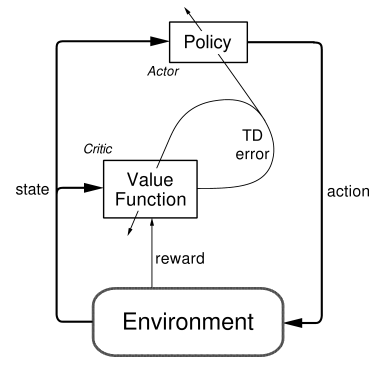
\includegraphics[scale=0.6]{fig/actor_critic.png}
    \caption{Actor-critic}
    \label{fig:actor_critic}
\end{figure}
%TODO Add emphatic TD ? 
\section{Deep Reinforcement Learning} %TODO Extend deep RL
Reinforcement learning algorithm showed great success on low dimensional tasks[CITATION HERE]. In recent years there has been significant advances in Supervised Learning to tackle high-dimensional data. Those methods are mainly based on deep neural network. A deep neural network is a an artificial neural network with several non linear layers. They are mainly trained using gradient descent and in particular back-propagation. 

Reinforcement learning algorithms combined with deep neural network as function approximation yields promising results on high dimensional problem (\citep{mnih2013playing,mnih2016asynchronous,schulman2017proximal}) such as Atari (\citep{bellemare2013arcade}) and Mujoco (\citep{todorov2012mujoco}). However, they appear to be very unstable and requires a number of \emph{tricks} to behave properly. We will describe 2 different algorithm Asynchronous Actor Critic ( A3C ~\citep{mnih2016asynchronous}) and Proximal Policy Optimzation (PPO ~\citep{schulman2017proximal}) and explain the tools used to make them stable. Both methods are based on actor critic formulation. 
\subsection{A3C}
One severe problem when using deep neural network as function approximation arise from the fact that the data is not Independently and Identically distributed. Indeed the samples received during the trajectory are highly correlated. This problem does not arise in supervised learning as it is possible shuffle the data randomly. It has been shown to cause severe learning problem in Reinforcement Learning. The first paper attempting to combine Deep Learning and Reinforcement Learning (DQN citation) used a replay buffer with Q-learning to combat this issue.

 In Asynchronous Advantage Actor-Critic \citep{mnih2016asynchronous}, the main idea is to propose a framework using asynchronous gradient descent for optimization of deep neural network controllers. This effectively decorrelate samples by having several agents running different trajectory at the same time. The data is then aggregated and one update is applied to all agents. This is effectively done by running several agents in parallel and using a batch of data to update the parameters. A diagram explaining the algorithm can be found in figure \ref{fig:a3c}.
\begin{figure}
    \centering
    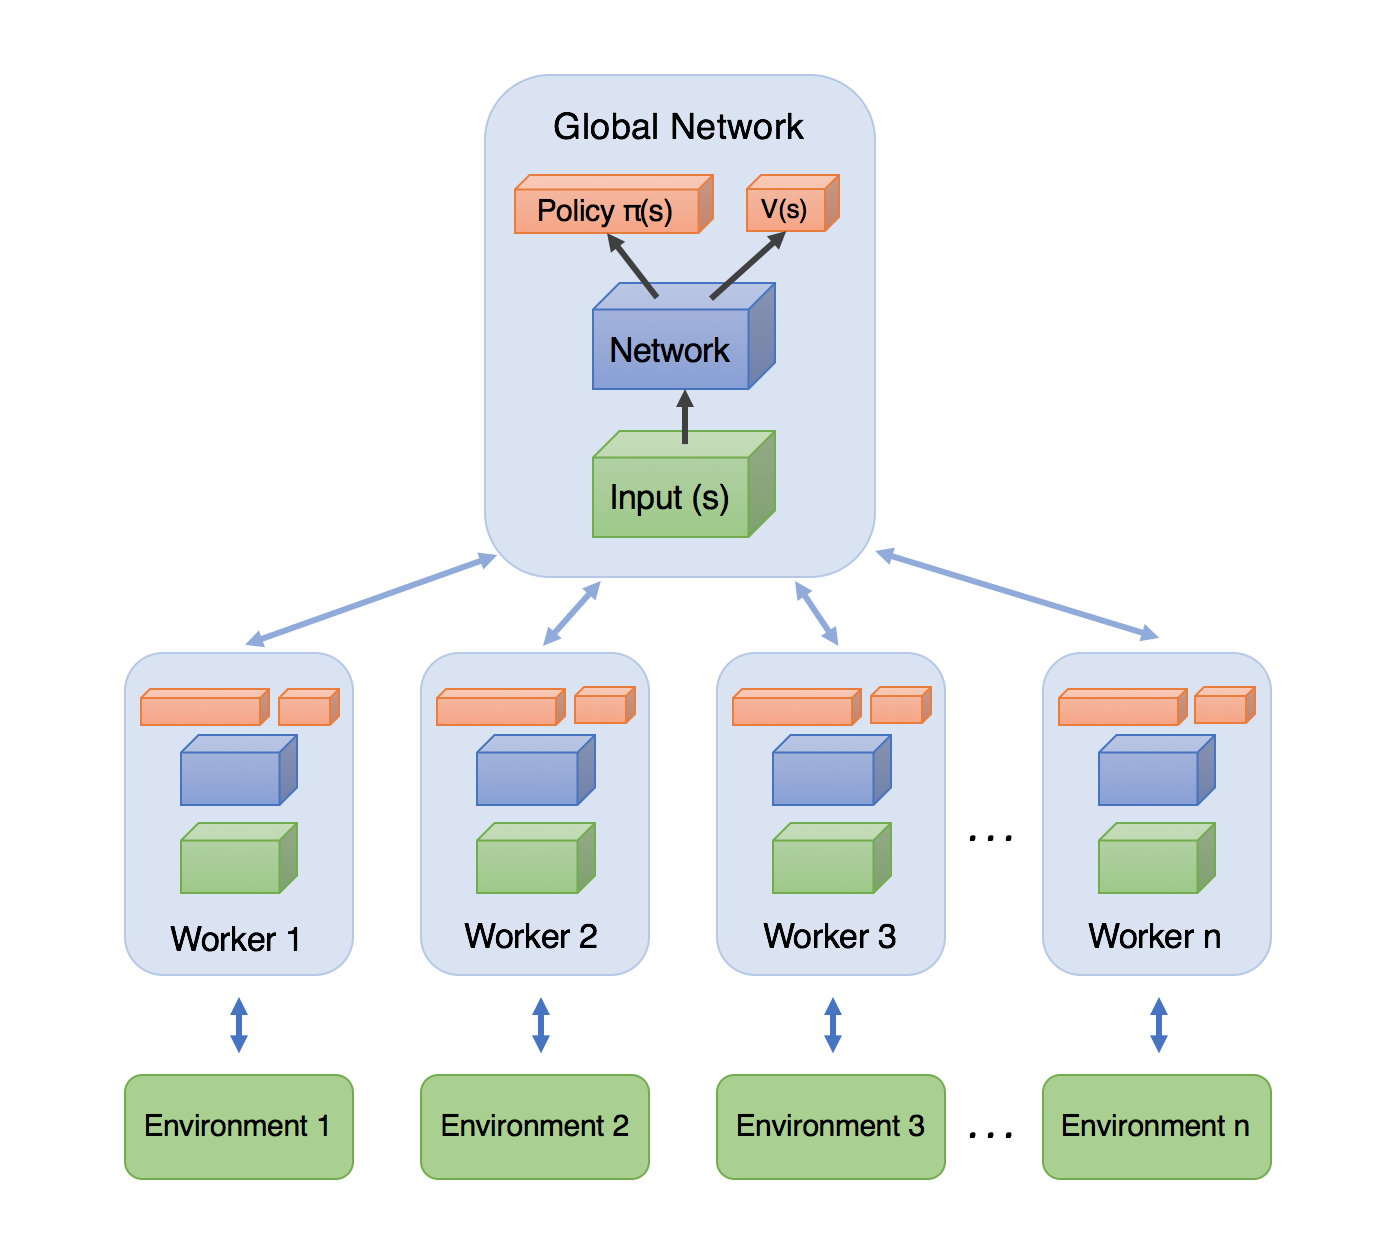
\includegraphics[scale=0.25]{fig/A3C.png}
    \caption[Asynchronous Advantage Actor-Critic]{A3C diagram(reproduced from this  \href{https://medium.com/emergent-future/simple-reinforcement-learning-with-tensorflow-part-8-asynchronous-actor-critic-agents-a3c-c88f72a5e9f2}{blog} with permission)}
    \label{fig:a3c}
\end{figure}
In the paper they demonstrate how their proposed method achieve performant policy on Atari domain and several continuous control tasks.
\subsection{PPO}
Another important issue in Reinforcement Learning is the one of non-stationarity of the data.
Proximal methods (\citep{schulman2017proximal,schulman2015trust}) alleviate this by limiting the update of the actor at each time step:
\begin{equation}
    \beta \text{KL}(\pi_{\text{old}},\pol_{\text{new}})
\end{equation}
where $\param$ control the magnitude of the regularization. This regularization has been found to be effective when combined with deep neural network as function approximator.



Regularization in Machine Learning is a cornerstone. Most models can be seen as bias/variance trade-off.
\section{Regularization} %TODO Write regularization text
Regularization in RL has been considered in several different perspectives. In this section we discuss the most popular one. 

\subsection{Spatial Regularization}
 One line of investigation focuses on regularizing the features learned on the state space (\citep{massoud2009regularized,petrik2010feature,pazis2011non,farahmand2011regularization,liu2012regularized,harrigan2016deep}). These approaches assume that nearby states in the state space have similar value. For example \citep{farahmand2011regularization} introduce Approximate Value iteration, designed to apply regularization technique to select value function estimators from rich function space.


%\subsubsection{Regularization of the function approximation}
%\citep{farahmand2011regularization}
%This thesis studies the reinforcement learning and planning problems that are modeled by a discounted Markov Decision Process (MDP) with a large state space and finite action space. We follow the value-based approach in which a function approximator is used to estimate the optimal value function. The choice of function approximator, however, is nontrivial, as it depends on both the number of data samples and the MDP itself. The goal of this work is to introduce flexible and statistically-efficient algorithms that find close to optimal policies for these problems without much prior information about them. The recurring theme of this thesis is the application of the regularization technique to design value function estimators that choose their estimates from rich function spaces. We introduce regularization-based Approximate Value/Policy Iteration algorithms, analyze their statistical properties, and provide upper bounds on the performance loss of the resulted policy compared to the optimal one. The error bounds show the dependence of the performance loss on the number of samples, the capacity of the function space to which the estimated value function belongs, and some intrinsic properties of the MDP itself. Remarkably, the dependence on the number of samples in the task of policy evaluation is minimax optimal. We also address the problem of automatic parameter-tuning of reinforcement learning/planning algorithms and introduce a complexity regularization-based model selection algorithm. We prove that the algorithm enjoys an oracle-like property and it may be used to achieve adaptivity: the performance is almost as good as the performance of the unknown best parameters. Our two other contributions are used to analyze the aforementioned algorithms. First, we analyze the rate of convergence of the estimation error in regularized least-squares regression when the data is exponentially beta-mixing. We prove that up to a logarithmic factor, the convergence rate is the same as the optimal minimax rate available for the i.i.d. case. Second, we attend to the question of how the errors at each iteration of the approximate policy/value iteration influence the quality of the resulting policy. We provide results that highlight some new aspects of these algorithms.

\subsection{Policy Regularization}
There exists several ways to regularize policy gradient method. The most comonly used in recent research is called entropy regularization \citep{neu2017unified,schulman2017proximal,bartlett2009regal}.
In policy gradient method, one successful approach consists of regularizing the entropy of your policy distribution \citep{neu2017unified}. Policy gradient methods will tend to converge to distributions with low entropy. By adding an entropy bonus, it encourages the policy to explore and often yields much better performance.
\begin{equation}
\begin{split}
    \pol &= \expect_{\pol}{r} + R(\pol)\\
    R(\pol) = \text{entrop}
\end{split}
\end{equation}
This sets of work \citep{schulman2017proximal,schulman2015trust} considers limiting the update of the policy gradient at each step to guarantee \emph{coherent} behavior. 


\subsection{Temporal Regularization}
Though no work explicitely considers the bias and variance induced of considering the past estimates, several work attempts to exploit this relationship to better performance.
\subsubsection{Natural value approximator}
The closest work to ours is possibly \citep{xu2017natural}, where they define natural value approximator by projecting the previous states estimates by adjusting for the reward and $\gamma$. Their formulation, while sharing similarity in motivation, yields different theory and algorithm in practice.
\subsubsection{Backward bootstrapping}
Backward bootstrapping method's can be seen as regularizing in feature space based on temporal proximity \citep{sutton2009fast,li2008worst,baird1995residual}
\subsection{Deliberation cost}
There exists between temporal regularization and option. Indeed having a high deliberation cost \citep{harb2017waiting} means that you smooth out your problem by having longer action. This can be seen as a bias variance trade off. 
\subsubsection{Temporal coherence}
Though it has been shown that exploiting \emph{temporal coherence} can benefit to tracking algorithms and thus help in meta-learning~\citep{sutton2007role}, this remains far from the setting considered in this work.

In this thesis we explicitely study the concept of temporal regularization and study the bias-variance induced.
USE THIS SPOT TO DO A TRANSITION TO TEMPORAL REGULARIZATION


\chapter{Temporal Regularization}
\label{chap:temporal}
\section{Value Based Temporal Regularization}
\label{sec:temp_reg}
%COMMENT(pierre-luc): "spatial" is not common terminology perhaps better to talk about regularization in feature space/state space, as in state abstraction vs temporal abstraction. Citations are also needed. Temporal regularization : could perhaps think of entropy-regularized work as a form of temporal regularization because it regularizes over pi_t and pi_{t+1}. You may also want to make it clear that "temporal regularization" is an expression coming from you, or otherwise provide citations. 
Regularization in the feature/state space, or \emph{spatial regularization} as we call it, exploits the regularities that exist in the observation (or state). In contrast, \emph{temporal regularization} considers the temporal structure of the value estimates through a trajectory. Practically this is done by smoothing the value estimate of a state using estimates of states that occurred earlier in the trajectory.
In this section we first introduce the concept of temporal regularization and discuss its properties in the policy evaluation setting. We then show how this concept can be extended to exploit information from the entire trajectory by casting temporal regularization as a time series prediction problem. 
\subsection{Definition}
Let us focus on the simplest case where the value estimate at the current state is regularized using only the value estimate at the previous state in the trajectory, yielding updates of the form % COMMENT(pierre-luc) : this sentence could be clearer. 
% Attempt: As a first step, we consider the case where the expected discounted return at a state also depends on the value at the previous step. 
% COMMENT(pierre-luc): You also need some more motivation as to why this particular form, especially the time-reversal aspect. Otherwise, it seems to be taken totally out of the blue. Why time-reversal matrix and not just P ? 
% COMMENT(pierre-luc) : "As a first step" suggests that you will introduce other forms of this operator in the paper. You do present the "time series" generalization, but don't develop it much further. So I would get rid of "first step", and start directly by explaining why incorporating previous values might be a good idea. 
\begin{equation}
    \begin{split}
        \Vr(s_{t}) &= \expect_{s_{t+1},s_{t-1} \sim \pi} [r(s_t) + \gamma ((1-\param)\Vr(s_{t+1}) + \param \Vr(s_{t-1}))]\\
         &= r(s_t) + \gamma (1-\param)\sum_{s_{t+1}\in \s} p(s_{t+1}|s_t)\Vr(s_{t+1})
         + \gamma \param \sum_{s_{t-1} \in \s}\frac{p(s_t|s_{t-1}) p(s_{t-1})}{p(s_t)} \Vr(s_{t-1}),
    \end{split}
\end{equation}
for a parameter $\param \in [0,1]$. It can be rewritten in matrix form as $\Vr = r + \gamma (((1-\param) P^{\pol} + \param \widetilde{P^{\pol}})\Vr) $, where $\widetilde{P^{\pol}}$ corresponds to the reversal Markov chain of the MDP.
We define a temporally regularized Bellman operator as:
\begin{equation}
\label{eqn:temp_reg_bellman_op}
    \regT v_{\param} = r + \gamma ((1-\param) P^{\pol}v_{\param} + \param \widetilde{P^{\pol}} v_{\param}).
\end{equation}
To alleviate the notation, we denote $P^{\pol}$ as $P$ and $\widetilde{P^{\pol}}$ as $\widetilde{P}$.
\begin{remark}
For $\param =0$, Eq.~\ref{eqn:temp_reg_bellman_op} corresponds to the original Bellman operator.
\end{remark}
We can prove that this operator has a unique fixed point, $\Vr^{\pol}$.
%COMMENT(pierre-luc): I would just splash Theorem 1 without stating Lemma 1 (which is just one line and isn't proved). You can instead mention it in the proof, and give a reference for this fact.
% \begin{lemma}
% \label{lem:stochastic_matrix_convex_combination}
% The convex combination of two row stochastic matrices is also row stochastic.
% \end{lemma}
\begin{theorem}
The operator $\regT$ has a unique fixed point $\Vr^{\pol}$ and $\regT$ is a contraction mapping.
\end{theorem}
\begin{proof}
We first prove that $\regT$ is a contraction mapping in $L_\infty$ norm. We have that
\begin{equation}
\begin{split}
    \norm{\regT u - \regT v}_{\infty} &= \norm{r+\gamma( (1-\param) Pu + \param \widetilde{P}u) - (r+\gamma( (1-\param) Pv + \param \widetilde{P}v))}_{\infty}\\
    &= \gamma \norm{((1-\param) P + \param \widetilde{P})(u-v)}_{\infty}\\
    &\leq \gamma \norm{u-v}_{\infty},
\end{split}
\end{equation}
where the last inequality uses the fact that the convex combination of two row stochastic matrices is also row stochastic (he proof can be found in the appendix).
%is obtained with Lemma~\ref{lem:stochastic_matrix_convex_combination}.
Then using Banach fixed point theorem, we obtain that $\Vr^{\pol}$ is a unique fixed point. 
\end{proof}
\begin{algorithm}[H]
\caption{Policy evaluation with temporal regularization}
\begin{algorithmic}[1]
    \STATE Input: $\pi,\alpha,\gamma,\param,\lambda$
    \STATE $p = V(s)$
    \FORALL{steps}
        \STATE Choose $a \sim \pi(\s)$
        \STATE Take action $a$, observe $r(s),s'$
        \STATE $\V(s) = r(s) + \gamma ( (1-\param) \V(s') + \param p) $
        \STATE $p = \V(s) $
    \ENDFOR
\end{algorithmic}
\label{alg:pol_eval_exp_smoothing}
\end{algorithm}

Furthermore the new induced Markov chain $(1-\param) P + \param \widetilde{P}$ has the same stationary distribution as the original $P$ (the proof can be found in the appendix).
\begin{lemma}
\label{cor:same_stationary_dist}
$P$ and $(1-\param) P + \param \widetilde{P}$ have the same stationary distribution $\mu \quad \forall \param \in [0,1]$.
\end{lemma}
%COMMENT(pierre-luc): $P$ and $(1-\param) : order is confusing. I would write something like:
% The stationary distribution induced by $(1-\param) P + \param \widetilde{P}$ is $\mu$: the stationary distribution under the original Markov chain $P$.


%COMMENT(pierre-luc): You first need to start this paragraph by saying that there is indeed a bias, because this is not something that you would expect from a "regular" policy evaluation operator. Then quickly reinsure the reader that this bias is not evil because the resulting operator as some desirable properties : a knob for variance reduction. 
\subsection{Bias}
In the policy evaluation setting, the bias between the original value function $\V^{\pol}$ and the regularized one $\V^{\pol}_{\param}$ can be characterized as a function of the difference between $P$ and its Markov reversal $\widetilde{P}$, weighted by $\param$ and the reward distribution.

%COMMENT(pierre-luc) : Minor notational preference in favor of "t" instead of "i". 
%COMMENT(pierre-luc): You need to say that these Neumann series converge. This follows from your contraction argument above. You can state Puterman corollary C.4 for the existence of the series and its inverse. 
%COMMENT(pierre-luc): A general statement for all LP norms ? If not, or generality is not needed, stick to more common sup/infinity norm. 
\begin{property}
Let $v^{\pol} = \sum_{i=0}^{\infty} \gamma^i P^i r$ and $v^{\pol}_{\param} = \sum_{i=0}^{\infty} \gamma^i ((1-\param) P + \param \widetilde{P})^i r$. We have that
\begin{equation}
    \begin{split}
        \norm{v^{\pol} - v^{\pol}_{\param}}_p &= \norm{\sum_{i=0}^{\infty} \gamma^i (P^i-((1-\param) P + \param \widetilde{P})^i) r}_p \\
        &\leq \sum_{i=0}^{\infty} \gamma^i \norm{ (P^i-((1-\param) P + \param \widetilde{P})^i) r}_p.
    \end{split}
\end{equation}
This quantity is naturally bounded for $\gamma < 1$.
\end{property}
\begin{remark}
Let $P^\infty$ denote a matrix where columns consist of the stationary distribution $\mu$.
By the property of reversal Markov chains and lemma \ref{cor:same_stationary_dist}, we have that $\lim_{i\rightarrow\infty} \Vert P^i r-P^\infty r \Vert \rightarrow 0$ and $\lim_{i\rightarrow\infty} \Vert ((1-\param)P+\param \widetilde{P})^i r-P^\infty r \Vert \rightarrow 0$, such that the Marvov chain $P$ and its reversal $(1-\param)P+\param \widetilde{P}$ converge to the same value. Therefore, the norm $\Vert  (P^i-((1-\param) P + \param \widetilde{P})^i) r \Vert_p$ also converges to 0 in the limit.
\end{remark}

\begin{remark}
It can be interesting to note that if the chain is reversible, meaning that $P = \widetilde{P}$, then the fixed point of both operators is the same, that is $v^\pol = v_\param^\pol$.
\end{remark}

\subsection{Variance}
If the chain is reversible than I can find a factor of 2 on the variance because you just get twice more sample. In the non reversible case same thing. If you were to be able to sample from the newly generated $P_{\param}$ then you would solve it half as fast. Could be a cool argument.
\subsection{Average reward case:} The temporally regularized MDP has the same average reward as the original one as it is possible to define the average reward \cite{tsitsiklis2002average} as a function of the stationary distribution $\pi$, the reward vector and $\gamma$ . This leads to the following property (the proof can be found in the appendix).

\begin{property}
For a reward vector r, the MDPs defined by the the transition matrices $P$ and $(1-\param) P + \param \widetilde{P}$ have the same average reward $\rho$.
\end{property}
Intuitively this means that temporal regularization only reweigh the reward on each state based on the Markov reversal while preserving the average reward.

%COMMENT(pierre-luc): You could also call this section "Higher Order Temporal Regularization". In RLS/ARMA/signal processing, I think they refer to the "order" of their filter when they incorporate older information. See LTI filters.
\subsection{Temporal Regularization as a time series prediction problem:}
It is possible to cast this problem of temporal regularization as a time series prediction problem and use richer models of temporal dependencies, such as exponential smoothing \cite{gardner2006exponential}, ARMA model~\cite{box94}, etc. We can write the update in a general form using $n$ different regularizers ($\widetilde{v_0},\widetilde{v_1}...\widetilde{v_{n-1}}$):
\begin{equation}
    \V(s_t) = r(s) + \gamma \sum_{i=0}^N [\param(i) \widetilde{\V}_i(s_{t+1})],
\end{equation}
where $\widetilde{\V}_0(s_{t+1}) = \V(s_{t+1})$ and $\sum_{i=0}^N \param(i) = 1$. For example, using exponential smoothing where $\widetilde{\V}(s_{t+1}) = (1-\lambda) \V(s_{t-1}) + (1-\lambda)\lambda \V(s_{t-2})...$, the update can be written in operator form as:
\begin{equation}
    \regT v = r + \gamma \bigg(\left(1-\param\right) Pv + \param \left(1-\lambda\right) \sum_{i=1}^{\infty} \lambda^{i-1} \widetilde{P}^i v\bigg),
\end{equation}
and a similar argument as Theorem 1 can be used to show the contraction property.

Using more powerful regularizers could be beneficial, for example to reduce variance by smoothing over more values (exponential smoothing) or to model the trend of the value function through the trajectory (trend adjusted model). An example a temporal policy evaluation with temporal regularization using exponential smoothing can be found in the appendix.
\begin{algorithm}[H]
\caption{Policy evaluation with exponential smoothing}
\begin{algorithmic}[1]
    \STATE Input: $\pi,\alpha,\gamma,\param,\lambda$
    \STATE $p = V(s)$
    \FORALL{steps}
        \STATE Choose $a \sim \pi(\s)$
        \STATE Take action $a$, observe $r(s),s'$
        \STATE $\V(s) =  r(s) + \gamma ( (1-\param) \V(s') + \param p) $
        \STATE $p = (1-\lambda)\V(s) + \lambda p$
    \ENDFOR
\end{algorithmic}
\label{alg:pol_eval_exp_smoothing}
\end{algorithm}
%COMMENT(pierre-luc) : It feels too disconnected from the flow. I would just move this to the conclusion as future work. 
\subsection{Control} 
Temporal regularization can be extended to control by  modifying the target of the value function (or the Q values) using temporal regularization. Experiments (Sec.~\ref{sec:expe:drl}) present an example of how temporal regularization can be applied within an actor-critic framework. The theoretical analysis of the control case is outside the scope of this paper.

\subsection{Temporal difference with function approximation}
It is also possible to extend temporal regularization using function approximation such as  semi-gradient TD \cite{sutton2017reinforcement}. 
%COMMENT(pierre-luc): Semi-gradient is a new terminology introduced in the draft of the new S&B textbook. Not found in 1998
Assuming a function $\V_{\theta}^{\param}$ parameterized by $\theta$, we can consider $r(s) + \gamma ((1-\param)\V_{\theta}^{\param}(s_{t+1}) + \param \V_{\theta}^{\param}(s_{t-1})) - \V_{\theta}^{\param}(s_t)$  as the target and differentiate with respect to $\V_{\theta}^{\param}(s_{t})$. An example of a temporally regularized semi-gradient TD algorithm can be found in the appendix.
%COMMENT(pierre-luc) : I would include this in the main text + pseudo-code. Important to show that the MDP formulation can be efficiently translated into a usable model-free algorithm. The time-reversibility would be a concern for me if I were to review this paper and it hadn't be addressed by this point yet. 


\begin{algorithm}[H]
\caption{Temporally regularized semi-gradient TD}
\begin{algorithmic}[1]
    \STATE Input: policy $\pi$,$\param$,$\gamma$
    \FORALL{steps}
        \STATE Choose $a \sim \pi(s_t)$
        \STATE Take action $a$, observe $r(s),s_{t+1}$
        \STATE $\theta = \theta + \alpha (r + \gamma((1-\param) \V_{\theta}(s_{t+1}) + \param \V_{\theta}(s_{t-1})) - \V_{\theta}(s_t))\nabla \V_{\theta}(s_{t}) $
    \ENDFOR
\end{algorithmic}
\end{algorithm}

\begin{property}
For a reward vector r, the MDP defined by the the transition matrix $P$ and $(1-\param) P + \param \widetilde{P}$ have the same average reward $\rho$.
\begin{equation}
    \frac{\rho}{1-\alpha} = \sum_i^{\infty}\gamma^i \pi^T r.
\end{equation}
\end{property}

\begin{lemma}
$P$ and $(1-\param) P + \param \widetilde{P}$ have the same stationary distribution $\mu \quad \forall \param \in [0,1]$.
\end{lemma}
\begin{proof}
It is known that $P^{\pol}$ and $\widetilde{P^{\pol}}$ have the same stationary distribution. Using this fact we have that
\begin{equation}
    \begin{split}
        \mu( (1-\param) P^{\pol} + \param \widetilde{P^{\pol}}) &=  (1-\param) \mu P^{\pol} + \param \mu \widetilde{P^{\pol}} \\
        &= (1-\param)\mu + \param \mu\\
        &= \mu.
    \end{split}
\end{equation}
\end{proof}

\begin{lemma}
\label{lem:stochastic_matrix_convex_combination}
The convex combination of two row stochastic matrices is also row stochastic.
\end{lemma}
\begin{proof}
Let e be vector a columns vectors of 1.
\begin{equation}
\begin{split}
       (\param P^{\pol} + (1-\param) \widetilde{P^{\pol}})e &= \param P^{\pol}e +  (1-\param) \widetilde{P^{\pol}}e \\
       &= \param e + (1-\param) e\\
       &= e.
\end{split}
\end{equation}
\end{proof}
\subsection{Connection with multi-step methods}

\section{Experiments}


We now presents empirical results illustrating potential advantages of temporal regularization, and characterizing its bias and variance effects on value estimation and control.



\subsection{Mixing time}
This first experiment showcases that the underlying Markov chain of a MDP can have a smaller mixing time when temporally regularized. The mixing time can be seen as the number of time steps required for the Markov chain to get \emph{close enough} to its stationary distribution. Therefore, the mixing time also determines the rate at which policy evaluation will converge to the optimal value function~\cite{baxter2001infinite}. 
%COMMENT(pierre-luc) : can also cite Puterman, spectral radius. Also, not just for control (you say "optimal") : also true for policy evaluation.
%COMMENT(pierre-luc): Mixing quickly is one thing, but mixing quickly and returning an answer not too far away from the actual answer (bias) is very important. When reading this paragraph, I would need to convince myself that this is not a vacuous demonstration, that the resulting fast-mixing chain is still somewhat related to the original problem.
We consider a synthetic MDP with 10 states where transition probabilities are sampled from the uniform distribution. Let $P^{\infty}$ denote a matrix where columns consists of the stationary distribution $\mu$. To compare the mixing time, we evaluate the error corresponding to the distance of $P^i$ and $\big((1-\param)P+\param \widetilde{P}\big)^i$ to the convergence point $P^{\infty}$ after $i$ iterations.
%
Figure~\ref{fig:mixing} displays the error curve when varying the regularization parameter $\param$. We observe a U-shaped error curve, that intermediate values of $\param$ in this example yields faster mixing time.
\begin{figure}
    \centering
    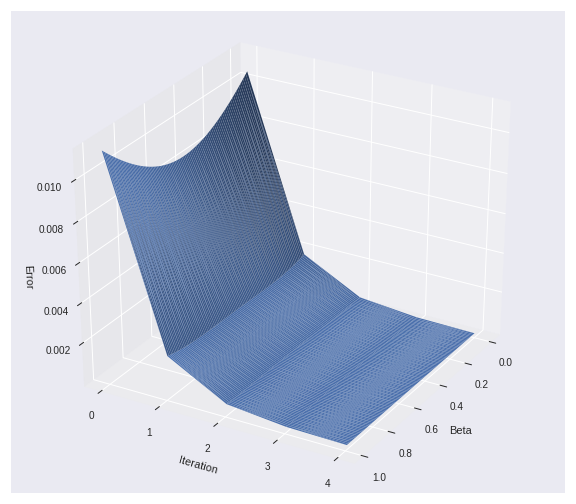
\includegraphics[scale=0.5]{fig/Markov_mixing.png}
    \caption{Distance between the stationary transition probabilities and the estimated transition probability for different values of regularization parameter $\param$.}
    \label{fig:mixing}
\end{figure}
One explanation is that transition matrices with extreme probabilities (low or high) yield poorly conditioned transition matrices. Regularizing with the reversal Markov chain often leads to a better conditioned matrix at the cost of injecting bias.
%COMMENT(pierre-luc) : poorly conditioned: you should compute the actual condition numbers to convince the reader that this is actually what is happening. 

\subsection{Bias}
\label{sec:expe:bias}

It is well known that reducing variance comes at the expense of inducing (smaller) bias.
%COMMENT(pierre-luc): citation still needed. You can perhaps cite general ML textbooks such as Hastie ESL or Bishop. You can also cite  Bertsekas (2012) and Satinder Singh and Kearns for bias-variance of TD(lambda).
This has been characterized previously (Sec.~\ref{sec:temp_reg}) in terms of the difference between the original Markov chain and the reversal weighted by the reward. In this experiment, we attempt to give an intuitive idea of what this means. More specifically, we would expect the bias to be small if values along the trajectories have similar values.
To this end, we consider a synthetic MDP with $10$ states where both transition functions and rewards are sampled randomly from a uniform distribution. In order to create temporal dependencies in the trajectory, we smooth the rewards of $N$ states that are temporally close (in terms of trajectory) using the following formula: $ r(s_t) = \frac{r(s_t) + r(s_{t+1})}{2}$.
Figure~\ref{fig:mod} shows the difference between the regularized and un-regularized MDPs as $N$ changes, for different values of regularization parameter $\param$.
\begin{figure}
    \centering
    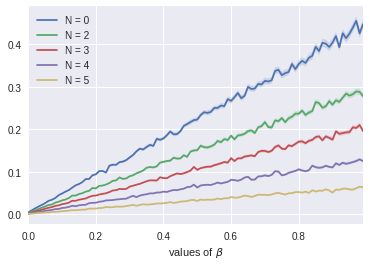
\includegraphics[scale=0.8]{fig/mod.png}
    \caption{Mean difference between $\Vr^{\pi}$ and $\V^{\pi}$ given the regularization parameter $\param$, for different amount of smoothed states $N$.}
    \label{fig:mod}
\end{figure}
We observe that increasing $N$, meaning more states get rewards close to one another, results into less bias. This is due to rewards putting emphasis on states where the original and reversal Markov chain are similar.

\subsection{Variance number 2}
You could use a random walk. The P is reversible to so no bias. Then compare the performance of monte carlo, TD and our thing. Should just be faster. In this case you want to compare with the number of samples used and try to show an increase of 2 folds. its like having double the sample link the variance from theory before

\subsection{Variance}
\label{sec:expe:variance}
% COMMENT(pierre-luc) : this should be emphasized earlier.
The primary motivation of this work is to reduce variance, therefore we now consider an experiment  targeting this aspect. Figure~\ref{fig:MDP} shows an example of a synthetic, three states MDP, where the variance of $S_1$ is (relatively) high.
\begin{figure}
    \centering
    \includegraphics[scale=0.7]{fig/Exp_2.png}
    \caption{Synthetic MDP where state $S_1$ has high variance.}
    \label{fig:MDP}
\end{figure}
We consider an agent that is evolving in this world, changing states following the stochastic policy indicated. We are interested in the error when estimating the optimal state value of $S_1$, $\V^*(S_1)$, with and without temporal regularization, denoted $\Vr^{\pi}(S_1)$, $\V^{\pi}(S_1)$, respectively.

Figure~\ref{fig:perf_MDP} shows these errors at each iteration, averaged over $100$ runs. We observe that temporal regularization indeed reduces the variance and thus helps the learning process by making the value function easier to learn.
\begin{figure}
    \centering
    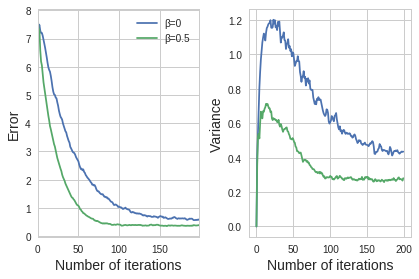
\includegraphics[scale=0.7]{fig/exp_2_result.png}
    \caption{Left plot showsabsolute difference between original ($\V^{\pi}(S_1)$) and regularized ($\Vr^{\pi}(S_1)$) state value estimates to the optimal value $\V^*(S_1)$. Right plot shows the variance of the estimates $\V$.}
    \label{fig:perf_MDP}
\end{figure}

\subsection{Propagation of the information}
We now illustrate with a simple experiment how temporal regularization allows the information to spread faster among the different states of the MDP. For this purpose, we consider a simple MDP, where an agent walks randomly in two rooms (18 states) using four actions (up, down, left, right), and a discount factor $\gamma=0.9$. The reward is $r_t=1$ everywhere and passing the door between rooms (shown in red on Figure~\ref{fig:room}) only happens 50\% of the time (on attempt). The episode starts at the top left and terminates when the agent reaches the bottom right corner. The sole goal is to learn the optimal value function by walking along this MDP (this is not a race toward the end).

Figure~\ref{fig:room} shows the proximity of the estimated state value to the optimal value with and without temporal regularization. The darker the state, the closer it is to its optimal value. The heatmap scale has been adjusted at each trajectory to observe the difference between both methods.
We first notice that the overall propagation of the information in the regularized MDP is faster than in the original one. We also observe that, when first entering the second room, bootstrapping on values coming from the first room allows the agent to learn the optimal value faster. This suggest that temporal regularization could help agents explore faster by using their prior from the previous visited state for learning the corresponding optimal value faster.

\begin{figure}
    \centering
    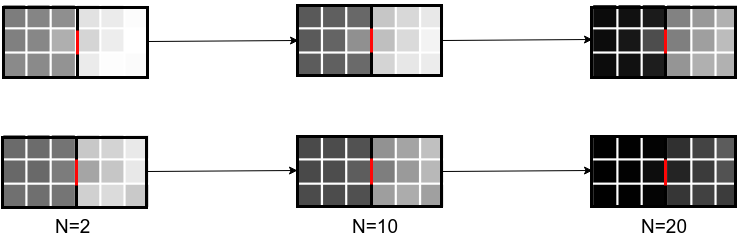
\includegraphics[scale=0.44]{fig/room.png}
    \caption{Proximity of the estimated state value to the optimal value after $N$ trajectories. Top row is the original room environment and bottom row is the regularized one ($\param = 0.5$). Darker is better.}
    \label{fig:room}
\end{figure}


\subsection{Noisy state representation}
\label{sec:expe:noisy_state}

The next experiment illustrates a major strength of temporal regularization, that is its robustness to noise in the state representation. This situation can naturally arise when the state sensors are noisy or insufficient to avoid aliasing.
\begin{figure}
    \centering
    
\includegraphics[scale=0.7]{fig/random_walk.png}
    \caption{Synthetic, one dimensional, MDP where the reward corresponds to the position of the agent in $[0, 1]$.}
    \label{fig:MDP_noisy}
\end{figure}
For this task, we consider the synthetic, one dimensional, continuous setting displayed in Figure~\ref{fig:MDP_noisy}. A learner evolving in this environment walks randomly along this line with a discount factor $\gamma=0.5$. Let $x_t\in [0,1]$ denote the position of the agent along the line at time $t$. The next position $x_{t+1} = x_t + a_t$, where action $a_t\sim\mathcal{N}(0, 0.1)$. The state of the agent corresponds to the position perturbed by a zero-centered Gaussian noise $\epsilon_t$, such that $s_t = x_t + \epsilon_t$, where $\epsilon_t\sim\mathcal{N}(0,\sigma^2)$ are i.i.d. When the agent moves to a new position $x_{t+1}$, it receives a reward $r_t = x_{t+1}$. The episode ends after 100 steps. In this experiment we model the value function using a linear model with a single parameter $\theta$. We are interested in the error when estimating the optimal parameter function $\theta^*$ with and without temporal regularization, that is $\theta^\pi_\param$ and $\theta^\pi$, respectively. In this case we use the TD version of temporal regularization presented at the end of Sec.~\ref{sec:temp_reg}.
\begin{figure}
    \centering
    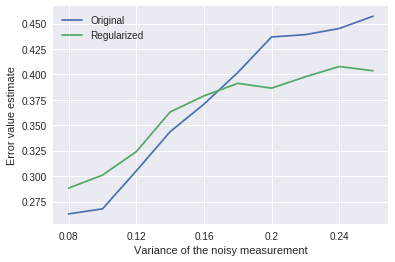
\includegraphics[scale=0.7]{fig/spatial_temporal.png}
    \caption{Absolute distance from the original ( $\theta^\pi$) and the regularized ($\theta^\pi_\param$) state value estimates to the optimal parameter $\theta^*$ given the noise variance $\sigma^2$ in state sensors.}
    \label{fig:perf_MDP_noisy}
\end{figure}
Figure~\ref{fig:perf_MDP_noisy} shows these errors, averaged over 100 repetitions, for different values of noise variance $\sigma^2$. We observe that as the noise variance increases, the un-regularized estimate becomes less accurate, while temporal regularization is more robust. This experiment highlights a case where temporal regularization is effective even in the absence of smoothness in the state space (which other regularization methods would target). This is further highlighted in the next experiments.



\subsection{Deep reinforcement learning}
\label{sec:expe:drl}

To showcase the potential of temporal regularization in high dimensional settings, we adapt an actor-critic based method (PPO \cite{schulman2017proximal}) using temporal regularization. More specifically, we incorporate temporal regularization as exponential smoothing in the target of the critic. 
% COMMENT(pierre-luc): Atari games: we evaluate the performance in the Arcade Learning Environment (ALE), citation Bellemare 2011 or 2013 ? 
We evaluate the performance on multiple Atari games, where we consider the following performance measure \cite{xu2017natural}:
\begin{equation}
\label{eqn:expe:drl_measure}
    \frac{\text{regularized} - \text{baseline}}{\text{baseline} - \text{random}}.
\end{equation}
%COMMENT(pierre-luc) : what is "baseline", plain PPO that you re-ran or other reported algorithm ?
The hyper-parameters for the temporal regularization are $\param = 0.2$ and a decay of $1\mathrm{e}^{-5}$. Those are selected on 7 games and 3 training seeds. All other hyper-parameters correspond to the one used in the PPO paper. Our implementation\footnote{The code can be found in the supplementary material.} is based on the publicly available OpenAI codebase~\cite{baselines}. The previous four frames are considered as the state representation~\cite{mnih2015human}.
For each game, $10$ independent runs ($10$ random seeds) are performed and the performance are reported in Figure~\ref{fig:graph_atari}. 


Figure~\ref{fig:graph_atari} shows that adding temporal regularization improves the performance on multiple games. This suggests that the regularized optimal value function may be smoother and thus easier to learn, even when using function approximation with deep learning. Also, as shown in previous experiments (Sec.~\ref{sec:expe:noisy_state}), temporal regularization being independent of spatial representation makes it more robust to mis-specification of the state features, which is a challenge in some of these games (e.g. when assuming full state representation using some previous frames).

\begin{figure}
    \centering
    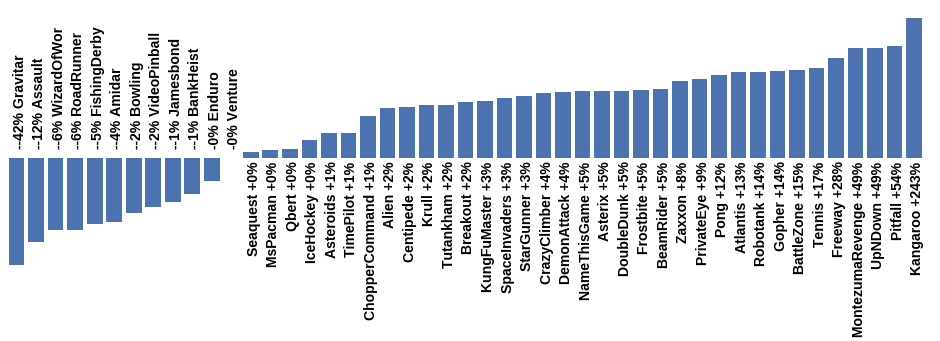
\includegraphics[width=13cm,height=4cm]{fig/bar_atari.png}
    \caption{Performance (Eq.~\ref{eqn:expe:drl_measure}) of a temporally regularized PPO on a suite of Atari games.}
    \label{fig:graph_atari}
\end{figure}

\begin{figure}
    \centering
    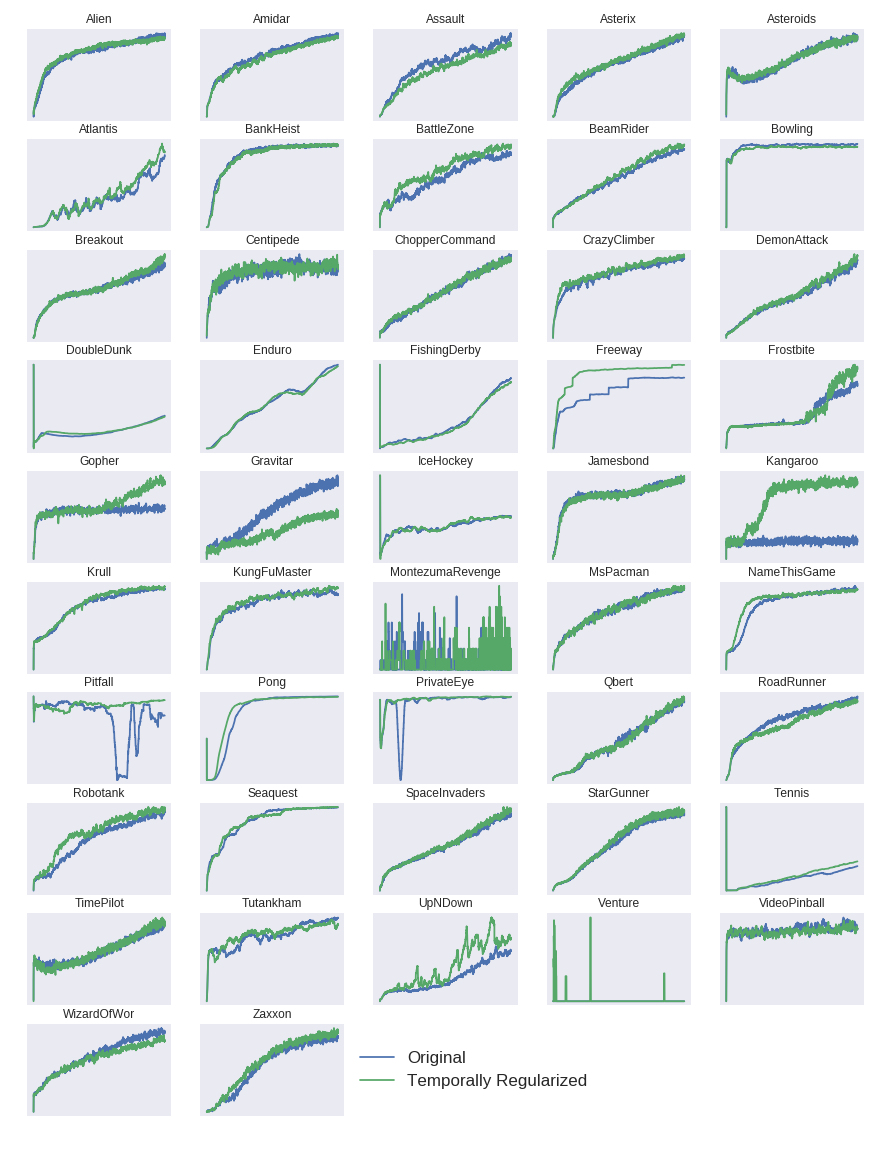
\includegraphics[scale=0.5]{fig/plot_atari.png}
    \caption{Average reward per episode on Atari games.}
    \label{fig:my_label}
\end{figure}
\section{Policy Gradient Temporal Regularization}

This idea is a continuation of the paper I wrote recently about what I call “Temporal Regularization”. The main intuition is to exploit previous estimate (v, q or pi’s) along the trajectory to reduce the variance of the current estimate. In particular in this project we are interested in policy gradient. We want to regularize the objective function by constraining the policy to be more "consistent" temporally 
\begin{equation}
\begin{split}
    R(\pi) = \beta ( \pi(a_{t-1}|s_{t-1}) - \pi(a_t|s_t)) \\
\end{split}
\end{equation}
It is possible to see this formulation as some kind of entropy regularization where the regularization is done in trajectory space compared to PPO ect… where it is done in policy space. Another perspective is to view $\pi$ as a time series and apply some entropy regularization to the prediction of the time series. Some of the advantages of doing this kind of regularization could be more consistent behavior in time, exploration, variance reduction.. \\
Theoretically we want to properly define this entropy using concepts of dynamical system and prove its potential convergence/convexity following the proof's used \cite{neu2017unified}.\\
More particularly in dynamical system there are several ways to define entropy. The community has not agreed on one in particularly form. Many of them are based on the kolmogorov sinai entropy. Intuitively they often define the entropy over each partition of your dynamical system and take a sup over that. In our case depending on how we average over the past we would implicitely define our partition function. This reference \url{http://prac.im.pwr.edu.pl/~downar/english/documents/entropy.pdf} is a good summary of the different form of entropy used. In particular I believe we can use something similar to the dynamical entropy explained in section 3.4.

Intuitively we want to minimize the "temporal entropy" when you are in an option/state of your dynamical system to get coherent behavior and maximize it when you change state/option. It is very related to option and deliberation cost \cite{harb2017waiting} as they minimize the entropy in an option by adding a cost to changing option. I believe deliberation cost can actually be cast as some kind of entropy minimization where your option defines the partition function. In our case by simply taking a combination of the previous step(or more) it is kind like implicitly defining an option with states that are around you.



\chapter{Recurrent Learning}
\label{chap:recurrent}

In the previous chapter we regularized the value estimate by adding a regularization term to the objective(target). In this chapter we explore explicitly averaging the value estimate using exponential smoothing.


This work proposes a method that attempts to address the following two aspects. 1) Minimization of the variance of the estimates through the \emph{trajectory}. 2) Learn a mechanism that emphasizes and de-emphasizes updates on relevant states.\\
Exponential smoothing (\cite{gardner1985exponential}) is one of the most widely used technique to reduce the variance of point estimates using \emph{previous observations}.
\begin{equation}
\begin{split}\label{smoothing}
    x_t &= \param s_t + (1-\param) x_{t-1}
\end{split}
\end{equation}
where $s_t$ is a signal, $x_t$ the averaged signal at time step $t$ and $\param$ a smoothing factor.
In time series data it is used to approximate the mean of a stream of data. This kind of smoothing has various names (\cite{polyak1992acceleration,kingma2014adam}) depending on the field it is used in.  Most quantities in reinforcement learning (Q values, state values, actions, etc) are estimated as point estimate ignoring previous estimates from the trajectory. We propose to use exponential smoothing in reinforcement learning on the trajectory. In other words, we propose to smooth the estimate of a state $s_t$ using the estimates of states $s_i$ that occur earlier in the trajectory ($i\geq t$). Intuitively, states that are temporally close to each other should have similar value.\\
However, exponential averaging can be biased if a sharp change(non-stationarity) is encountered in the trajectory, like falling off a cliff. To alleviate this issue a common technique used is to set $\param_t$ the exponential smoothing factor as a state or time dependent. In Recurrent Neural Networks, it is possible to view LSTM (\cite{hochreiter1997long}) and GRU (\cite{chung2014empirical}) as several non linear exponential smoothing functions. The key ingredient is the gating mechanism(state dependent $\param_t$) used to update the hidden cell. The capacity to ignore information allows the cell to focus only on important information. This can also be found in semi-iterative method used to solve linear system of equations. (\cite{golub1961chebyshev}) finds the optimal $\param_t$ using Chebyshev polynomials. In this work we explore a new method that attempts to learn a state dependent smoothing factor $\param$. We show how it relates to existing methods and exploits similar properties such as emphatic TD (\cite{sutton2016emphatic,mahmood2015emphatic}). 
The contributions of the paper are as follows:
\begin{itemize}
    \setlength\itemsep{0.1em}
    \item Propose a new way to estimate value function in reinforcement learning by exploiting the estimates along the trajectory.
    \item Provide asymptotic convergence guarantee in the tabular setting under some smoothness assumption.
    \item Derive a learning rule for a state dependent $\param$.
    \item Perform a set of experiments in tabular and continuous settings to evaluate its strengths and weaknesses.
\end{itemize}





\section{Recurrent Learning in Reinforcement Learning}
\label{RLRL}
In this work, we propose to estimate the value function using the estimates along the trajectory. The value of a state $s$ at time step $t$ is given by:
\begin{equation}
\label{value}
\begin{split}
    \vr(s_t) &= \param_t \Vt(s_t) + (1 - \param_t) (\vr(s_{t-1})) \\ 
\end{split}
\end{equation}
where $\vr$ is an exponential smoothing of $\Vt$. $\vr$ is a function parametrized by $\theta$ and $\param$. We consider $\param$ to be fixed for each state in this section and relax the assumption later. For a given set of state dependant $\param(s_t) = \param_t$, the goal is to find a set of parameters $\theta$ minimizing,
\begin{equation}\label{loss_beta}
    \text{min}_{\theta} \mathcal{L}(\theta) = \text{min}_{\theta} \expect_{\pol} [(V^{\pol} - \vr)^2]
\end{equation}
In contrast to traditional methods that attempts to minimize Eq. \ref{simple_loss} we explicitly enforce temporal consistency by finding $\theta$ that minimizes Eq. \ref{loss_beta}.
By taking the derivative with respect to Eq. \ref{loss_beta} we obtain the following update:
\begin{equation}
\begin{split}
    \theta &= \theta + \alpha \delta_t  \nabla_{\theta} \vr (s_t) \\
\end{split}
\end{equation}
where $\delta_t = V^{\pol}(s_t) - \vr(s_t)$.
 The gradients of $\vr$ can be expressed in a recursive form:
\begin{equation}
    \nabla_{\theta} \vr (s_t) = \param_t \nabla_{\theta} \Vt + (1-\param_t) \nabla_{\theta} \vr (s_{t-1})
\end{equation}
For computational reason, it is possible to approximate the gradient $\nabla_{\theta}\vr (s_{t})$ using a recursive \emph{eligibility} trace:
\begin{equation}
\label{trace}
    e_t = \param_t \nabla_{\theta} \Vt (s_t) + (1-\param_t) e_{t-1}
\end{equation} 
The potential bias induced by this approximation are discussed later in the paper.
We present Recurrent Temporal Difference(RTD) in Algorithm \ref{RTD}.
\begin{algorithm}[H]
\caption{Recurrent Temporal Difference, RTD(0)}
\begin{algorithmic}[1]
    \label{RTD}
    \STATE Input: $\pi$,$\param$,$\gamma$,$\theta$
    \STATE Initialize: $\vr(s_0) = \Vt(s_0)$ and $e_0 = \nabla_{\theta} \Vt(s_0)$
    \STATE Output: $\theta$
    \FORALL{t}
        \STATE Choose $a \sim \pi(s_t)$
        \STATE Take action $a$, observe $r(s_t),s_{t+1}$
        \STATE $\vr(s_t) = \param_t \Vt(s_t) + (1-\param_t) (\vr (s_{t-1})$
        \STATE $e_t = \param_t \nabla_{\theta} \Vt(s_t) + (1-\param_t) e_{t-1}$
        \STATE $\delta_t = r(s_t) + \gamma \Vt(s_{t+1}) - \vr(s_t)$
        \STATE $\theta = \theta + \alpha \delta_t e_t $
    \ENDFOR
\end{algorithmic}
\end{algorithm}
In practice, $\vr(s_0)$ is initialized with the value of the first state $\Vt(s_0$). We can understand our algorithm better when we intuitively interpret its effect in the \emph{extreme cases} ($\param=\{0,1\}$). We consider TD(0) in a tabular setting for simplicity. First, consider a state $s_t$ where $\param(s_t) = 0$. The value of this state is frozen at the initialization point and is never updated. This is because the trace as defined in Eq. \eqref{trace} is $e_t = e_{t-1}$ making such a state \emph{ineligible} for the update. The error received at this state is used to update the previous states as per their \emph{eligibility} in $e_{t-1}$. This means that for a state $s_t$ with $\param(s_t)=1$, $\Vt(s_t)$ is updated at every time step $t+n$ until another state with $\param(s_{t+n}) = 1$ is encountered.

For any $i \leq t$ where $\param_i \in (0,1]$, it is possible to express $\vr(s_t)$ as:
\begin{equation}
\begin{split}\label{decompose}
    \vr(s_t) &= \Vt(s_i) - \Delta_t(s_i) \\
    \Delta_t(s_i) &= (1-C_t(s_i))(\Vt(s_i) - \widetilde{V}_t(s_i) ) 
\end{split}
\end{equation}
where $C_t(s_i) = \param_i \prod_{p=i+1}^t (1-\param_p)$, $\widetilde{V}_t(s_t)$ is a convex combination of all $\Vt$ encountered in the trajectory except $\Vt(s_i)$ weighted by their respective contribution($\param$) to the estimate $\vr(s_t)$. For example, if we consider updating $\Vt(s_2)$ at $t=3$ and have the following $\param_1 = 0.9,\param_2 = 0.1,\param_3 = 0.1$. The value of $\widetilde{V}_3(s_2)$ will be mainly composed of $\Vt(s_1)$. The main component of the error will be $V^{\pol}(s_3) - \Vt(s_1)$. We take an example with $t=3$ and consider $i=2$:
\begin{equation}
    \begin{split}
        \vr(s_3) &= \param_3 \V(s_3) + (1-\param_3)\param_2 \V(s_2) + (1-\param_3)(1-\param_2)  \V(s_1)\\
        &= \V(s_2) - (1-(1-\param_3)\param_2)(\V(s_2) - \frac{\param_3 \V(s_3) + (1-\param_3)(1-\param_2)  \V(s_1)}{(1-(1-\param_3)\param_2)})\\
        &= \V(s_2) - (1-(1-\param_3)\param_2)(\V(s_2) - \widetilde{V}_t(s_i))
    \end{split}
\end{equation}
To see that $\widetilde{V}$ is a convex combination of the all the $\V$ encountered along the trajectory weight by $\param$ except $V(s_2)$ it suffices to see that:
\begin{equation}
    \begin{split}
        & \frac{\param_3  + (1-\param_3)(1-\param_2)  }{(1-(1-\param_3)\param_2)} = 1 \\
        &\equiv \param_3  + (1-\param_3)(1-\param_2)  = (1-(1-\param_3)\param_2) \\
        &\equiv \param_3 + (1-\param_3)\param_2 + (1-\param_3)(1-\param_2) = 1
    \end{split}
\end{equation}
where the last line is true because $\param \in (0,1]$Every update to $\Vt(s_i)$ made during the trajectory at time step $t$ can be decomposed as follows:
\begin{equation}
\label{decompose}
\begin{split}
    \Vt(s_i) = \Vt(s_i) + \alpha e_t(s_i) ( V^{\pol}(s_t) + \Delta_t(s_i) - \Vt(s_i))
\end{split}
\end{equation}
$\Delta_t(s_i)$ can be interpreted as a regularization term composed of the difference between $\Vt(s_i)$ and $\widetilde{V}_t(s_i)$. In practice, one can observe an increase in the magnitude of this term with a decrease in \emph{eligibility}. This suggests that the biased updates contribute less in the learning. Bounding the magnitude of $\Delta$ to ensure contraction is the key concept used in this paper to ensure asymptotic convergence.

\subsection{Asymptotic convergence}
Consider a tabular setting with TD(0). The main idea is to cast recurrent learning as an asynchronous stochastic approximation (\cite{tsitsiklis1994asynchronous}) with an additional regularization term. By bounding the magnitude of this term we show that the operator is a contraction. The algorithm is asynchronous because the eligibility trace updates only certain states at each time step.

Following the decomposition in Eq. \ref{decompose} we can recover the stochastic approximation formulation described in Eq. \ref{stoch} with the following operator $\T^{\param}: \mathbb{R^{|\mathbb{S}|}} \rightarrow \mathbb{R^{|\mathbb{S}|}}$:
\begin{equation}
    \T^{\param} V(s_i) = \expect_{\pol}[r_t + \gamma \Vt(s_{t+1}) + \Delta_t(s_i)]
\end{equation}
for all states $s_i$ with $\param_i \in (0,1]$.
We consider the following assumptions to prove convergence.
The first assumption deals with the ergodic nature of the Markov chain. It is a common assumption in theoretical reinforcement learning that guarantees infinitely many visits to all states thereby avoiding chains with transient states.
\begin{assumption}
The Markov chain is ergodic.
\end{assumption}
The second assumption concerns the relative magnitude of the maximum and the minimum reward. It is a key element that allow us to bound the magnitude of the regularization term. 
\begin{assumption}
\label{a_rew}
We define $R_{\max}$ and $R_{\min}$ as the maximum and minimum reward in a MDP. The relative magnitude between them is bounded by a factor of D such that:
\begin{equation}
\begin{split}
    DR_{\text{max}}  &\leq R_{\text{min}}  \\
    D &> \gamma \\
    R_{\text{min}} &\geq 0\\
\end{split}
\end{equation}
where $D \in (0.5,1]$ is a constant to be defined based on $\gamma$.
\end{assumption}
This is the most restrictive assumption of the proof. Relaxation to this assumption is proposed in the discussions. Although assumption \ref{a_rew} is restrictive in theory we never observed a divergence in tabular and deep RL settings that we considered.

As mentioned earlier, the key component of the proof is to control the magnitude of the term in Eq. \ref{decompose}: 
$\Delta_t(s_i) = (1-C_t(s_i))(\Vt(s_i) - \widetilde{V}_t(s_i))$. As the eligibility of this update gets smaller the magnitude of the term gets bigger. This suggests that not updating certain states whose eligibility is less than the threshold \emph{C} can help mitigate biased updates.
Depending on the values of $\gamma$ and $D$ we may need to set a threshold $C$ to guarantee convergence.
\begin{theorem}
\label{contraction_theorem}
Define $V_{\max} = \frac{R_{\max}}{1-(\gamma+(1-D))}$ and $V_{\min} = \frac{R_{\min}}{1-(\gamma-(1-D))}$. $\T^{\param}: X \rightarrow X$ is a contraction operator if the following holds:
\begin{itemize}
    \item Let $X$ be the set of $\Vt$ functions such that $\forall s \in \mathbb{S} \quad  V_{\min} \leq \Vt(s) \leq V_{\max}$.  The functions $\Vt$ are initialized in $X$.
    \item For a given $D$ and $\gamma$ we select $C$ such that $\Delta \leq (1-C)(V_{\max}-V_{\min}) \leq (1-D)V_{\min}$
\end{itemize}
\end{theorem}
\begin{proof}
The first step is to prove that $\T^{\param}$ maps to itself for any noisy update $\widetilde{\T^{\param}}$. 
From 2) we know that
$(1-C) V_{\max} - V_{\min} < D V_{\min} \leq D V_{\max}$ we can then deduce that
\begin{equation}
    \begin{split}
        \widetilde{\T^{\param}}\V(s) &\leq R_{\max} + \gamma V_{\max} +(1-C)(V_{\max} - V_{\min}) \\
        &\leq R_{\max} + (\gamma+(1-D)) V_{\max} \\
        &\leq V_{\max}
    \end{split}
\end{equation}
and
\begin{equation}
    \begin{split}
        \widetilde{\T}^{\param}\V(s) &\geq R_{\min} + \gamma V_{\min} + (1-C)(V_{\min} - V_{\max})\\
        &\geq R_{\min} + (\gamma-(1-D)) V_{\min}\\
        &\geq V_{min}\\
    \end{split}
\end{equation}
The next step is to show that $\T^{\param}$ is a contractive operator:
\begin{equation}
\begin{split}
    &\norm{\T^{\param}V - \T^{\param}U}_{\infty}\\
    &\leq \max_{s,s'}\expect_{\pol}[\gamma V(s) + \Delta^V(s') - (\gamma U(s) + \Delta^U(s'))] \\
    &\leq \max_{s,s'}\expect_{\pol}[\gamma (V(s)-U(s)) + (1-D)(V(s') -U(s'))]\\
    &\leq \max_{s}\expect_{\pol}[((1-D)+\gamma)(V(s) - U(s))]\\
    &\leq ((1-D)+\gamma) \norm{V - U}_{\infty}
\end{split}
\end{equation}
and from the assumption we know that $(1-D)+\gamma < 1$.
\end{proof}
 We provide an example to decide a choice on $C$ based on $\gamma$ and $D$.
 To select C based on $\gamma$ and $D$ it suffice to solve analytically for:
\begin{equation}
\begin{split}
    &(1-C)(V_{\max} - V_{\min}) \leq (1-D)V_{\min} \\
    &\equiv (1-C)\frac{R_{\max}}{1-(\gamma + (1-D)} \leq ((1-D)+(1-C)) \frac{R_{\min}}{1-(\gamma - (1-D)}\\
    &\equiv \frac{(1-C)(1-(\gamma-(1-D)))}{(1-(\gamma + (1-D))((1-D)+(1-C)} R_{\max}\leq R_{\min} \\
    &\equiv \frac{D(1-C)(1-(\gamma-(1-D)))}{(1-(\gamma + (1-D))((1-D)+(1-C)} R_{\min} \leq R_{\min}
\end{split}
\end{equation}
which is satisfied only if:
\begin{equation}
\begin{split}
    \frac{D(1-C)(1-(\gamma-(1-D)))}{(1-(\gamma + (1-D))((1-D)+(1-C)} &\leq 1
\end{split}
\end{equation}
As an example for $D = 0.8$ and $\gamma = 0.5$ any $C\geq 0.33$ satisfies this inequality.

We can guarantee that $\Vt$ converges to a fixed point of the operator $\T^{\param}$ with probability one using theorem 3 of (\cite{tsitsiklis1994asynchronous}). 
We now discuss the assumptions of theorem 3 in (\cite{tsitsiklis1994asynchronous}) 
\paragraph{Assumption 1:} Allows for delayed update that can happen in distributed system for example. In this algorithm all $\V$'s are updated at each time step $t$ and is not an issue here.
\paragraph{Assumption 2: } As described by (\cite{tsitsiklis1994asynchronous}) assumption 2 ``allows for the possibility of deciding whether to update a particular component $x_i$ at time $t$, based on the past history of the process.''. This assumption is defined to accommodate for $\epsilon$-greedy exploration in Q-learning. In this paper we only consider policy evaluation hence this assumptions holds.
\paragraph{ Assumption 3:} The learning rate of each state $s \in \mathbb{S}$ must satisfy Robbins Monroe conditions such that there exists $C \in \mathbb{R}$:
\begin{equation}
    \begin{split}
        \sum_{i=0}^{\infty} \alpha_t(s) 
e_t(s) &= \infty \quad \text{w.p.1}\\
        \sum_{i=0}^{\infty} (\alpha_t(s) e_t(s))^2 &\leq C      \end{split}
\end{equation}
This can be verified by assuming that each state gets visited infinitely often and an appropriate decaying learning rate based on $\#_s$ (state visitation count) is used (linear for example). 
\paragraph{Assumption 5:} This assumption requires $\T$ to be a contraction operator. This has been proven in theorem 1 of this paper.

Theorem \ref{contraction_theorem} in its current form is not general enough to provide convergence in all tabular settings. It is meant to provide a first way to prove convergence for recurrent learning and lead the way to more refined analysis. Such extensions are discussed later in the paper.

% Function Approx Stuff. Commenting it out now.



%EXPLAIN HERE JUMPY N-STEP RETURN USING THE EXAMPLE\\

\subsection{State dependent $\param$}
As mentioned earlier, state dependent $\param$ are responsible for the success of certain techniques. For instance, the success of LSTM (\cite{hochreiter1997long}) can be attributed to the gating(state dependent smoothing) mechanism.In this section we consider $\param_{\omega}$ where $\param_t$ is estimated with a set of parameters $\omega$. There is a natural way to estimate $\param$ in our formulation as given below.

\begin{equation}\label{classic_loss}
    \text{min}_{\param} \expect_{\pol}\norm{V^{\pol}-\vr}_{2}
\end{equation}

In practice, this compares the estimate $\Vt(s_t)$ and $\vrb(s_{t-1})$ to $V^{\pol}$ and gives more weight to the one that is closer among the two. This differs from the greedy approach (\cite{white2016greedy}) to set $\lambda$ as we don't explicitly need to consider the variance of the return.
As an example, we derive an analytic form of gradient of $\param_{\omega} = \sigma(\omega_{s_t})$ where $\omega_{s_t}$ is a scalar. Taking the derivative of Eq. \ref{classic_loss}, gives the following update rule:
\begin{equation}
\begin{split}
    \omega_{s_t} &= \omega_{s_t} + \alpha ( \sigma (\omega_{s_t})(1 -  \sigma(\omega_{s_t}) (V^{\pol}(s_t) -\vr(s_t) )(\Vt(s_t) - \vr(s_{t-1}))).  \label{beta_ur}
\end{split}
\end{equation}
A full derivation of Eq. \ref{beta_ur} is given below and a table illustrating the behavior of $\param$ following the loss described.

We wish to find $\param = \sigma(\omega)$ minimizing the loss : 

\begin{align}
    \min \ \ \frac{1}{2}(V^{\pol}(s_t) - \vrb(s_t))^2  \\
\end{align}
Taking the derivative of the R.H.S of 2 gives

\begin{align}
    \frac{d}{d\omega_{s_t}} \ \ &\bigg( \frac{1}{2}(V^{\pol}(s_t) - \vrb(s_t))^2  \bigg) =(V^{\pol}(s_t) - \vrb(s_t)) \big(\frac{d (V^{\pol}(s_t) - \vrb(s_t))}{d\omega_{s_t}} \big) 
     \big) )  \ \ \ 
\end{align}
We know that 
\begin{equation}
\frac{d}{d\omega} \sigma(\omega_{s_t})=\sigma(\omega_{s_t})(1 - \sigma(\omega_{s_t}))
\end{equation}
and 
\begin{equation}
\begin{split}
	\frac{d}{d\sigma(\omega_{s_t})} (V^{\pol}(s_t) - \vrb(s_t)) &= \frac{d}{d\sigma(\omega_{s_t})} \bigg(\sigma(\omega_{s_t})\V(s_t) + \big(1 - \sigma(\omega_{s_t})\big)\vrb(s_{t-1}) - V^{\pol}(s_t)\bigg)\\
	 &= \V(s_t) - \vrb(s_{t-1})
\end{split}
\end{equation}
Therefore, 
\begin{align}
    &\frac{d}{d\omega} \ \ \bigg( \frac{1}{2}(V^{\pol}(s_t) - \vrb(s_t))^2 + \lambda \sigma(\omega_{s_t}) \bigg) =\\
    &(V^{\pol}(s_t) - \vrb(s_t)) (\V(s_t) - \vrb(s_{t-1}))\bigg(\sigma(\omega_{s_t})(1 - \sigma(\omega_{s_t}))\bigg)
     + \lambda \bigg(\sigma(\omega_{s_t})(1 - \sigma(\omega_{s_t}))\bigg)  = \\
     &\bigg(\sigma(\omega_{s_t})(1 - \sigma(\omega_{s_t}))\bigg) \bigg((V^{\pol}(s_t) - \vrb(s_t))(\V(s_t) - \vrb(s_{t-1})) \bigg)
\end{align}
\begin{table}
\begin{center}
\begin{tabular}{ c|c c } 
  & \small{$V^{\pol}(s_t)>\vr(s_t)$} & \small{$V^{\pol}(s_t)<\vr(s_t)$} \\ 
   \hline
 \small{$\V(s_t)>\vr(s_{t-1})$} & $\param \uparrow$ &  $\param \downarrow$ \\ 
 \small{$\V(s_t)<\vr(s_{t-1})$} & $\param \downarrow$ & $\param \uparrow$  \\ 
\end{tabular}
\end{center}
\end{table}
One caveat to consider with this update rule concerns the magnitude of $V$. In practice, to avoid the saturation of the sigmoid unit, the loss needs to be in a similar range $\sim [0,1]$. This can be mitigated by scaling the loss or cutting the gradients above a certain magnitude as done in PPO. (\cite{schulman2017proximal}).
A second caveat is that the gradient with respect to $\omega$ could be expanded further to include previous time steps. This is ignored in the tabular setting to favor simplicity of the update. However, this gradient is considered in deep reinforcement learning setting due to the strength of automatic differentiation.
We now give an example of how this error can behave. Consider a situation in which one of the two scenarios could happen. In the first scenario, we see a spike due to a noisy reward or an error in the function approximator or a noise in the state representation. In the second scenario, this spike arise due to a sparse reward from the environment. This is illustrated in the figure \ref{fig:noise}. In the first scenario, $\vr$ is a better estimate of the expected discounted return than a 1-step estimate. Therefore, the algorithm learns to lower $\param$ around the spike to smooth out the trajectory hence lowering the variance. However, in the second scenario, $\vr$ becomes biased and the algorithm learns to trust its current estimate, driving $\param$ to 1. This is a classic bias variance trade-off, where the state dependant $\param$ can help us lower the bias induced. There exists an interesting connection to explore between $\lambda$ and $\param$ as $\lambda$ return is a better target to learn $\param$. This relationship is explored further in the experimental section of the paper.

\begin{figure}[h]
    \centering
    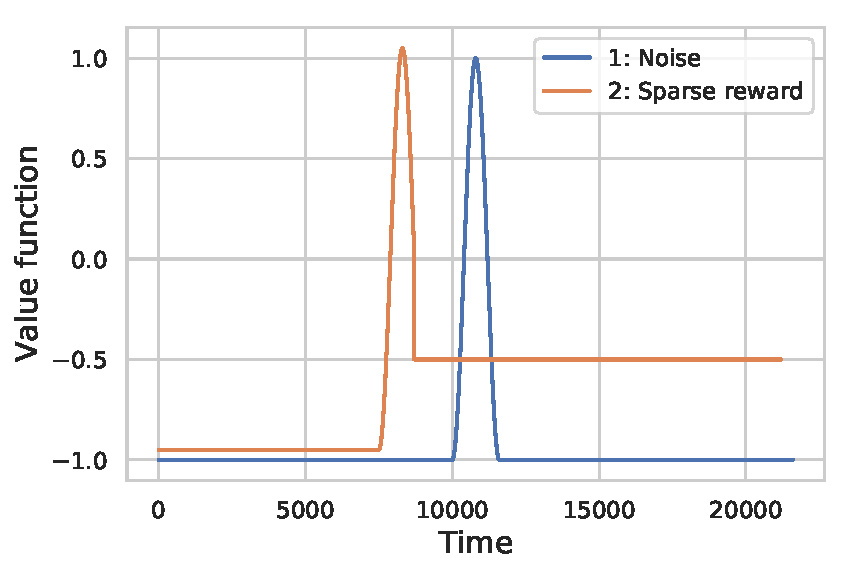
\includegraphics[scale=0.5]{fig/noise_sparse.pdf}
    \caption{Noise versus sparse reward}
    \label{fig:noise}
\end{figure}

\subsection{Adjusting for the reward}
In practice many environments in reinforcement learning have either a constant negative reward or a constant positive reward at every time step. In order to account for those rewards we propose an alternative formulation where $\vr$ accounts for the reward that was just seen:
\begin{equation}
\label{value_reward}
    \vr(s_t) = \param_t \Vt(s_t) + (1 - \param_t) (\vr(s_{t-1}) - r_{t-1}) 
\end{equation}

The decision on the choice of formulation to use will depend on the environment considered. In the case where $\param$ is restricted to $\param = \{0,1\}$, the updates on a state $V(s_i)$ can be interpreted as an undiscounted N-step return:
\begin{equation}\label{undiscounted}
        \delta_t = V^{\pol}(s_t) + \sum_{p=i}^{t-1} r_p - \Vt(s_i).
\end{equation}
From a theoretical perspective, convergence of this formulation can be considered by modifying the bound on $\Delta$ to accommodate the reward. This is left as a future work. 

\section{Related work}
Recurrent learning shares similarities with many algorithms in reinforcement learning. The most important similarity is with respect to $\lambda$ return (\cite{sutton1998reinforcement,dayan1992convergence}). There is often a debate of explicit versus implicit modelling in reinforcement learning and supervised learning from a conceptual perspective. $\lambda$ return is a way to implicitly enforce temporal coherence through the trajectory. In this paper, we propose a method to \emph{explicitly} enforce the temporal coherence using recurrent learning. Furthermore, recurrent learning yields a natural way to estimate an emphasis function whereas setting $\lambda$ efficiently still remains an open problem. In practice both $\lambda$ return and recurrent learning may be needed to properly enforce temporal coherence. The capacity to ignore states also share some similar motivations to semi-Markov decision process (\cite{puterman1990markov}) and Temporal Value Transport (\cite{TVT}). Temporal Value Transport attempts to exploit similar ideas that recurrent learning does. It does so in a different manner. In particular, Temporal Value Transport is based on a discrete attention mechanism using threshold values in contrast to our continuous $\param$ \emph{attention} mechanism. This yields very different algorithms and theory in practice. As mentioned earlier, there exists similarities with emphatic TD (\cite{mahmood2015emphatic}) in the sense that it emphasizes or de-emphasizes the update done to a state based on $\param$. One key difference with emphatic TD is that the interest is decayed across all the states using $\gamma$, whereas in this work it is based on the interest of the future states. Our formulation is driven by the success of \emph{forgetting} and \emph{ignoring} in supervised learning. Furthermore, learning the emphasis function is not explored in (\cite{mahmood2015emphatic}). Our work also relates to Temporal Regularization (\cite{thodoroff2018temporal}) that smooth the target of temporal difference methods using previous values of the trajectory. Although sharing similar motivation, the algorithms proposed are different. In particular, learning \emph{smoothing} coefficient is not considered. Finally, (\cite{xu2017natural}) proposes a mechanism to adaptively learn to use previous estimates. In practice, this is done by considering an \emph{auxiliary loss} between the target and the previous estimate in contrast with the setup considered here. Furthermore, the theoretical properties(convergence) of their algorithm is not considered.


\section{Experiments}
\begin{figure}[h]
    \centering
    \includegraphics[width=10cm]{fig/toy_MDP.png}
    \caption{Simple chain MDP. The dotted line in the figure indicates multiple states in between shown states.}
    \label{fig:toy MDP}
\end{figure}
We consider the simple chain MDP described in figure \ref{fig:toy MDP} to demonstrate our method. This MDP has three chains connected together to form a \emph{Y}. Each of the 3 chains (left of $S_1$, right of $S_2$, right of $S_3$) is made up of a sequence of states. The agent starts at $S_0$ and navigates through the chain. At the intersection, $S_1$, there is a $0.5$ probability to go top or bottom. The chain on the top has a reward of $+1$ at the last state and the chain on the bottom has a reward of $-1$. Every other transition has a reward of $0$, unless specified otherwise.\\
\subsection{Bias Variance trade-off}
\begin{figure}[h]
    \centering
    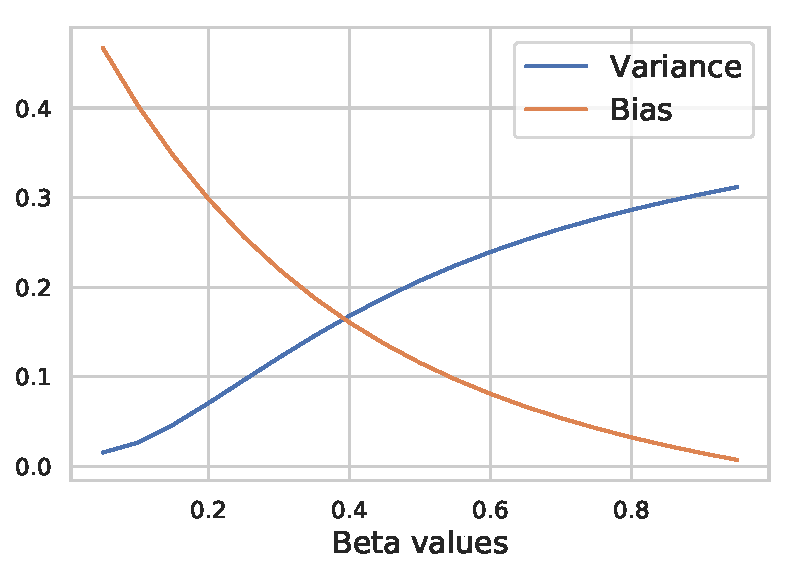
\includegraphics[scale=0.6]{fig/beta_bias_variance.pdf}
    \caption{Bias variance trade off of $\vr$ throughout the trajectory using exponential smoothing}
    \label{fig:bias_variance}
\end{figure}
It is possible to decompose policy evaluation into two sub tasks. The first one is given a set of functions $\Vt$, the goal is to estimate optimal values of states along the trajectory. The second task is to compare this set of functions that can be estimated by either considering the loss in Eq. \ref{simple_loss} or the recurrent loss in Eq. \ref{loss_beta}. In this experiment, we focus on the former task to demonstrate the bias variance trade-off induced by exponentially smoothing the values over the trajectory. This is shown in figure \ref{fig:bias_variance}. 

The value function $\Vt$ is learned using TD(0) with the loss described in Eq. \ref{simple_loss}. For all states $s_i \in \mathbb{S}$ we average the bias and the variance of $\vr(s_i)$ over 500 episodes. We define the \emph{bias} as $\norm{\Vt(s_i) - \vr(s_i)}_{2}$. Intuitively, it is the distance between the estimate $\Vt(s_i)$(used as optimal values for this experiment) and the exponentially smoothed estimate $\vr(s_i)$. We experiment with a range of fixed $\param$'s. We observe a decrease in bias and an increase in the variance as the $\param$ increases. In other words, the value of each state is forced to be close to the values in the past when $\param$ is low. This results in smooth values along the trajectory but biased due to their reliance on the past. As $\param \to 1$ we tend to be close to classic TD setting. One important note, to accurately demonstrate the bias variance trade-off induced by using exponential smoothing, we use the same learning mechanism for both $\vr$ and $\Vt$, namely the loss in Eq. (\ref{simple_loss}). This choice is necessary to have a proper comparison; choosing different losses would induce different fixed points and make the comparison difficult.



\subsection{Partially observable setting}
\begin{figure}[h]
    \centering
    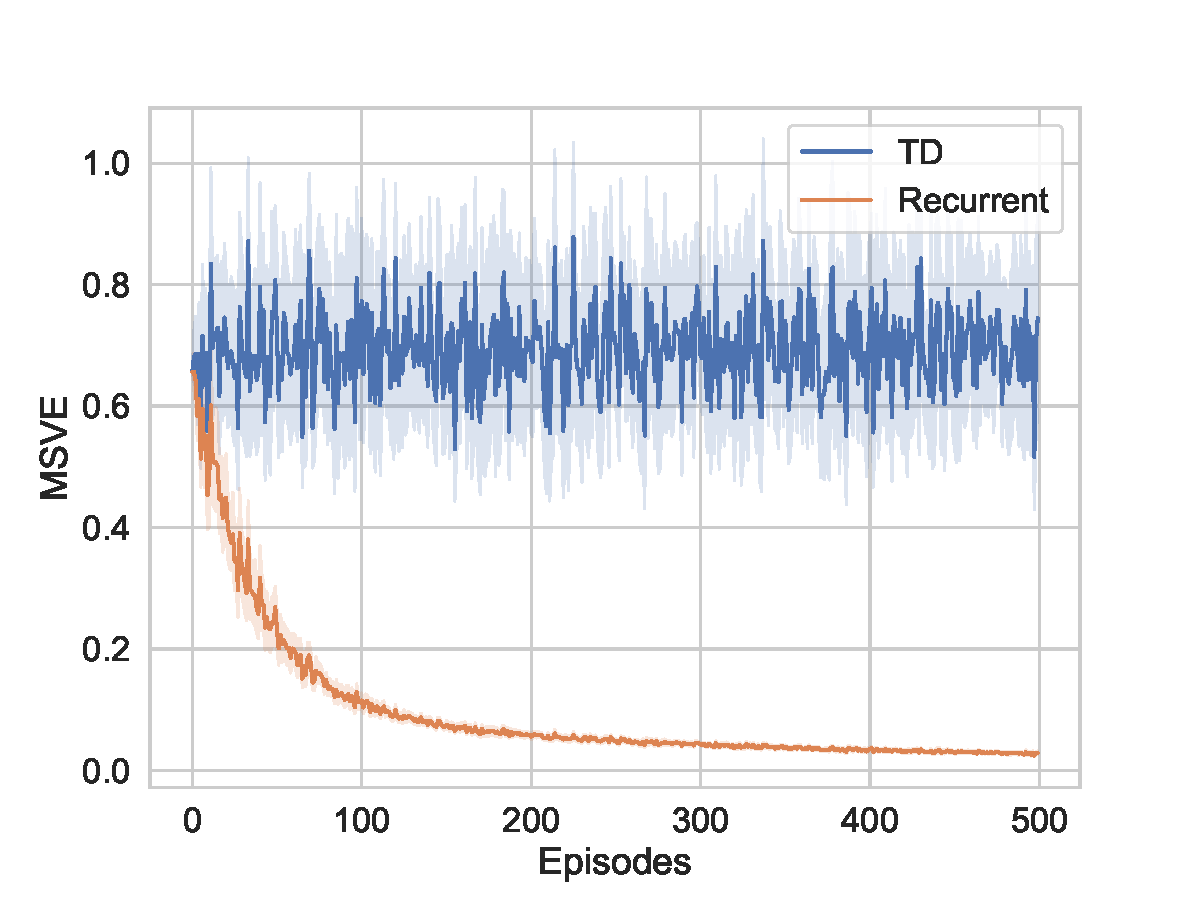
\includegraphics[scale=0.6]{fig/POMDP.pdf}
    \caption{TD versus Recurrent TD on aliased Y-chain}
    \label{fig:pomdp}
\end{figure}
Next, we explore the capacity of recurrent learning to solve a partially observable task. In particular, we consider the case where some states are aliased (share a common representation). The representation of the state following $S_4$ and $S_5$ in figure \ref{fig:toy MDP} is aliased. The goal of this environment is to correctly estimate the value of the aliased state $V^{\pol}(S_4)=0.81,V^{\pol}(S_5)=-0.81$(due to the discounting and the length of each chain being 5). When TD($\lambda$) is used to estimate the values for these states, the values of states $S_4$ and $S_5$ is close to 0 as the reward at the end of the chain is $+1$ and $-1$. However, when learning $\param$, recurrent learning achieve almost no error in the estimate of the aliased state as illustrated in figure \ref{fig:pomdp}. To understand this result the first thing to realize is that $\param=0$ on the aliased state as the previous values along the trajectory are a better estimate of the future along the same chain compared to the actual estimate of the aliased state. As $\param \to 0$, $\vr(S_4)$ and $\vr(S_5)$ tends to rely on the previous estimate $V(S_2)$ and $V(S_3)$ which are accurate. We see that learning to ignore certain states can sometimes be enough to solve correctly an aliased tasks in contrast to a traditional POMDP method that would attempt to infer the belief state. The results displayed in figure \ref{fig:pomdp} are averaged over 20 random seeds. The learning rate used is $0.05$, $\gamma = 0.9$ and $\lambda = 0.9$.
\subsection{Deep reinforcement learning}

In this experiment, we modify the critic of Proximal Policy Optimization (PPO)~(\cite{schulman2017proximal}) to use recurrent learning. We modify the critic to estimate the value function parametrized by $\theta$ using recurrent learning. We add a separate network parametrized by $\omega$ (same architecture as PPO) to learn a state dependant $\param$. The following loss is minimized:
\begin{equation}\label{ppo_loss}
    \min_{\param,\omega} \expect_{\pol}(\Vt^{\lambda}-\vr)^2)
\end{equation}
where the target $\Vt^{\lambda}$ is the generalized advantage function (\cite{schulman2015high}). Using an automatic differentiation library (Pytorch \cite{paszke2017automatic}) we differentiate Eq.\ref{ppo_loss} through the modified estimate to learn the $\theta$ and $\omega$. The hyperparameters of PPO are not modified. Due to the batch updates in PPO, obtaining the trajectory information to create the computational graph can be costly. As a result, we cut the backpropagation after $N$ timesteps in a similar manner to truncated backpropagation through time (\cite{williams1995gradient}). The learning rate for the $\param$ network, L1 regularization coefficient of $\param$ and number of backpropagation steps were obtained using hyperparameter search and details can be found in the appendix \ref{deep_RL_appendix}. We used a truncated backprop of $N=5$ in our experiments as found no empirical improvements for $N=10$. However, we expect in some settings(e.g. long term credit assignment) backprop further can be advantageous. The motivation to regularize $\param$ to be sparse comes from bounded rationality. Our brain has limited capacity and only updating the value at key states is a desirable property. This parameter plays a similar role as the deliberation cost in option (\cite{harb2018waiting}). The best performing set of parameters included a regularization parameter of $0.5$ supporting this hypothesis. The performance reported are averaged over 20 different random seeds. \footnote{The base code used to develop this algorithm can be found here (\cite{pytorchrl}). The code for Recurrent PPO can be found in the supplementary material}.

\subsubsection{Performance}
\begin{figure}
    \centering
    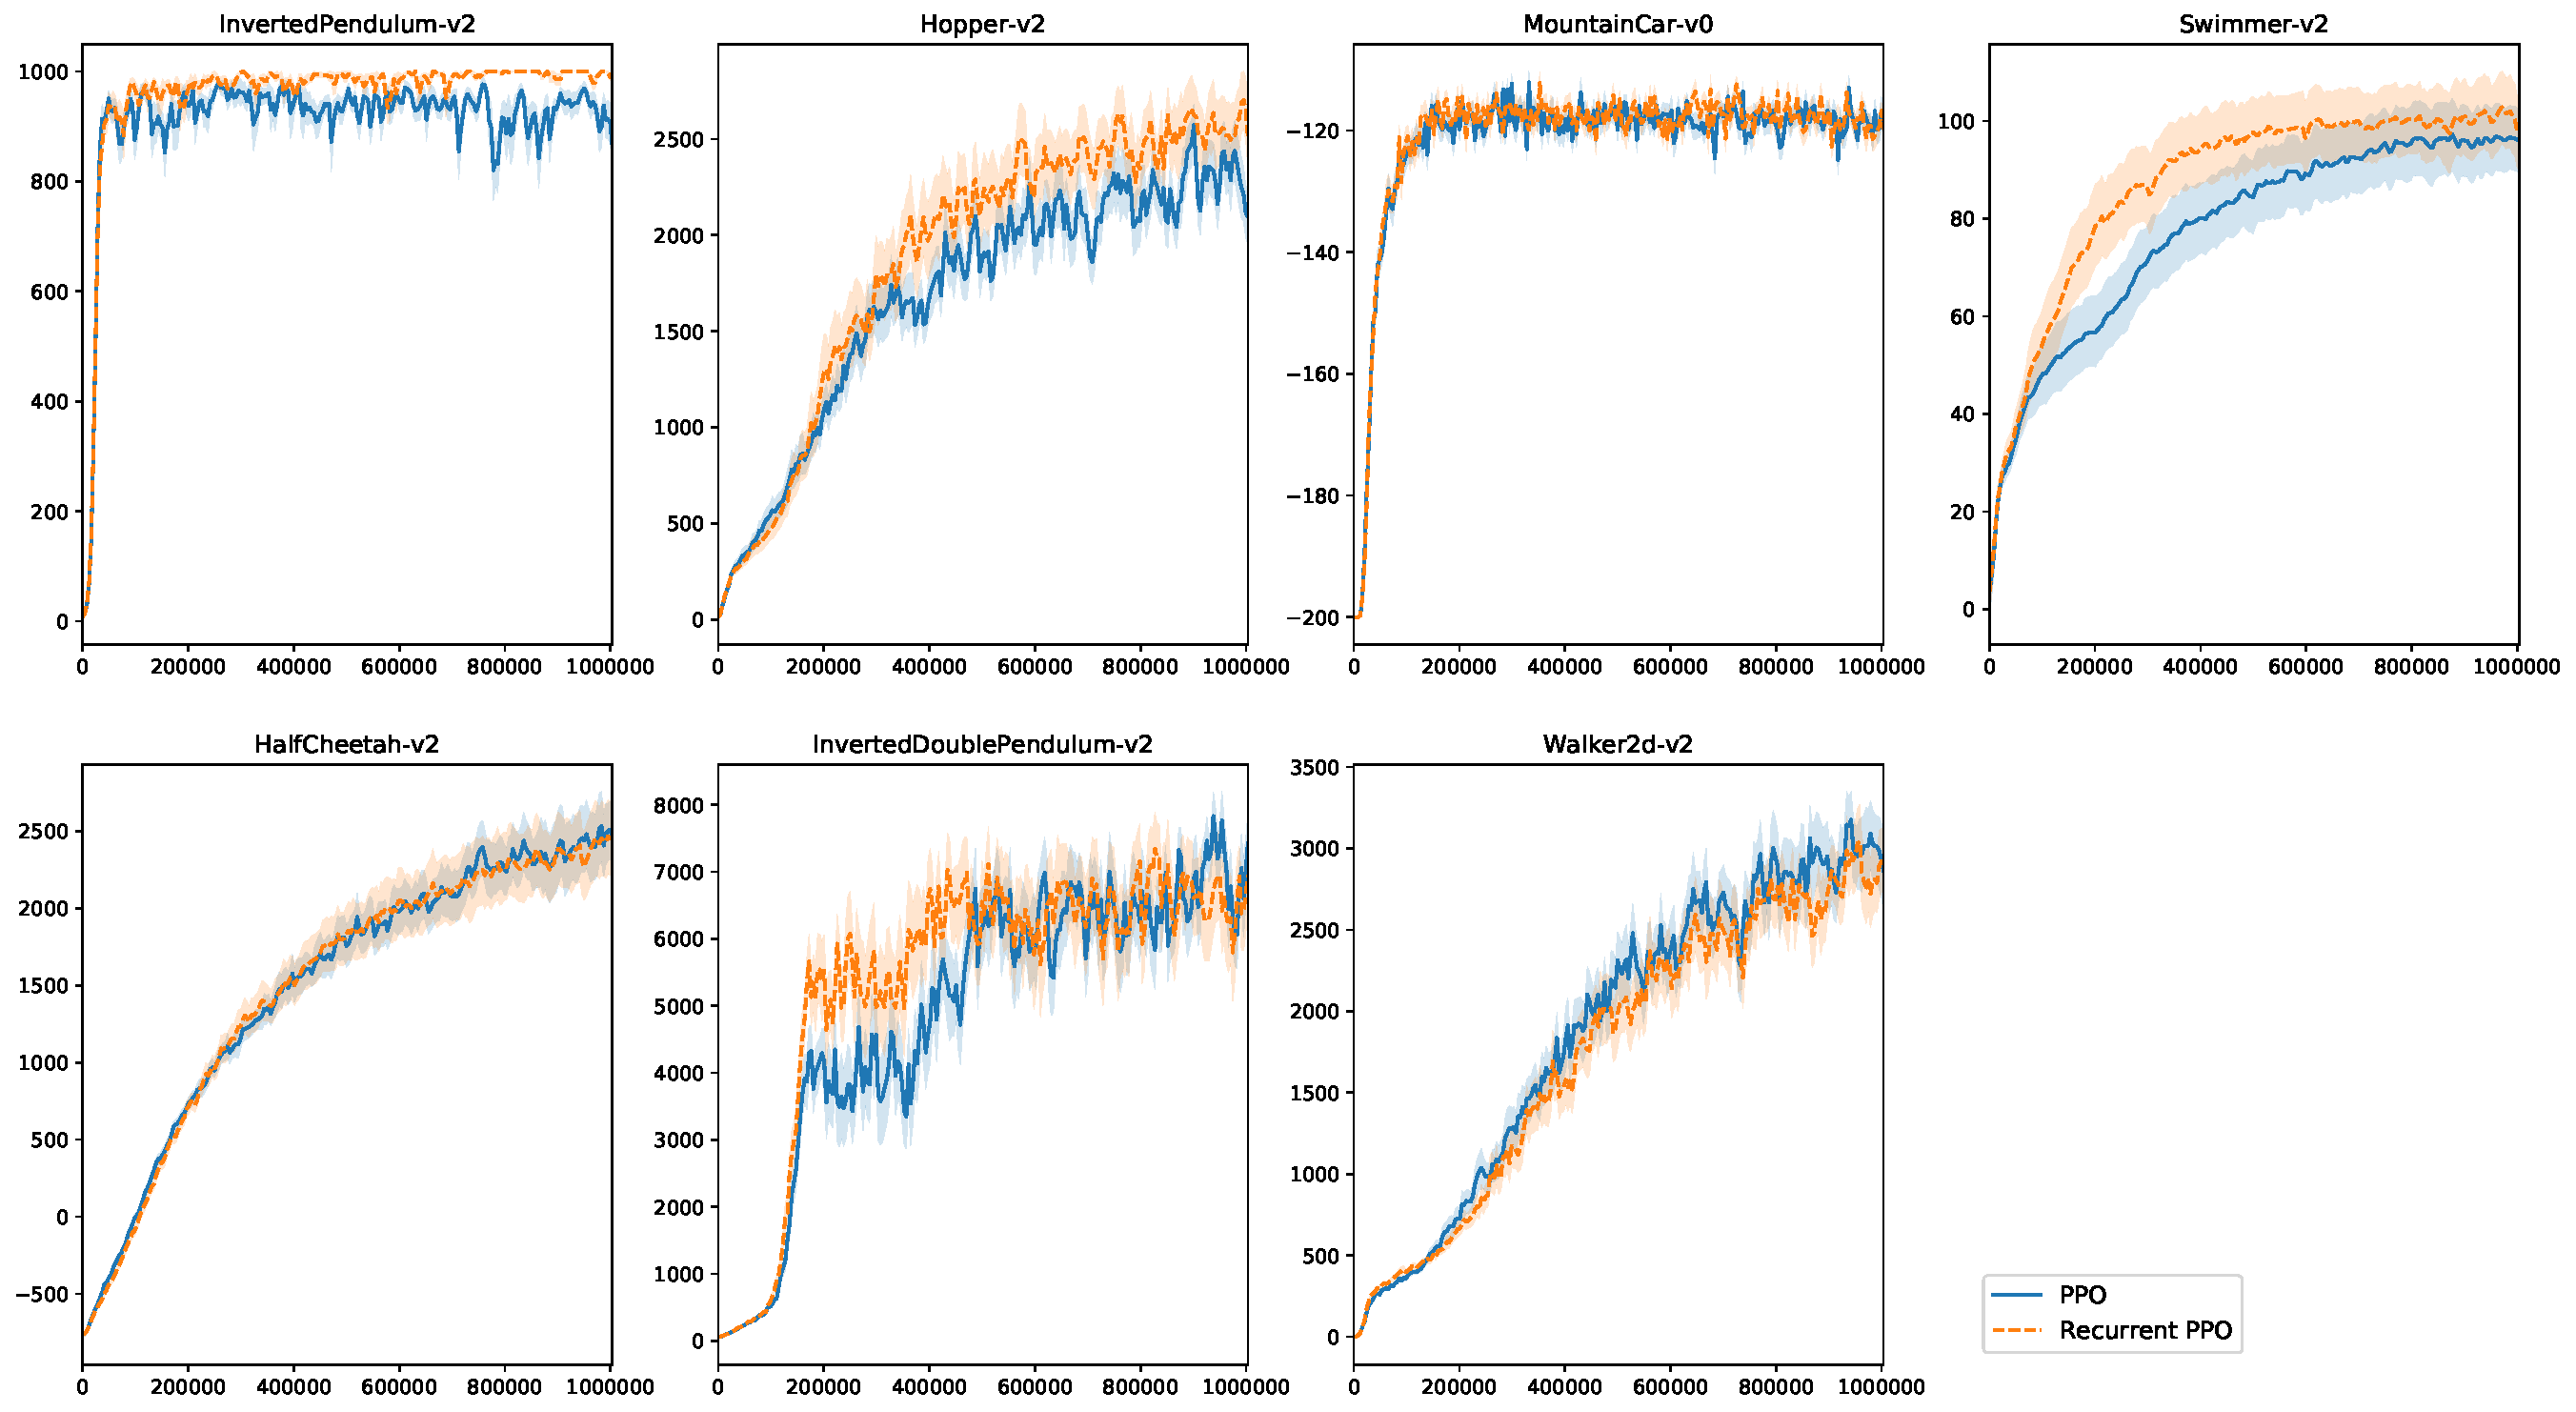
\includegraphics[scale=0.34]{fig/full_mujoco.pdf}
    \caption{Mean reward using recurrent PPO on Mujoco domains}
    \label{fig:full_mujoco}
\end{figure}
\begin{figure}
    \centering
    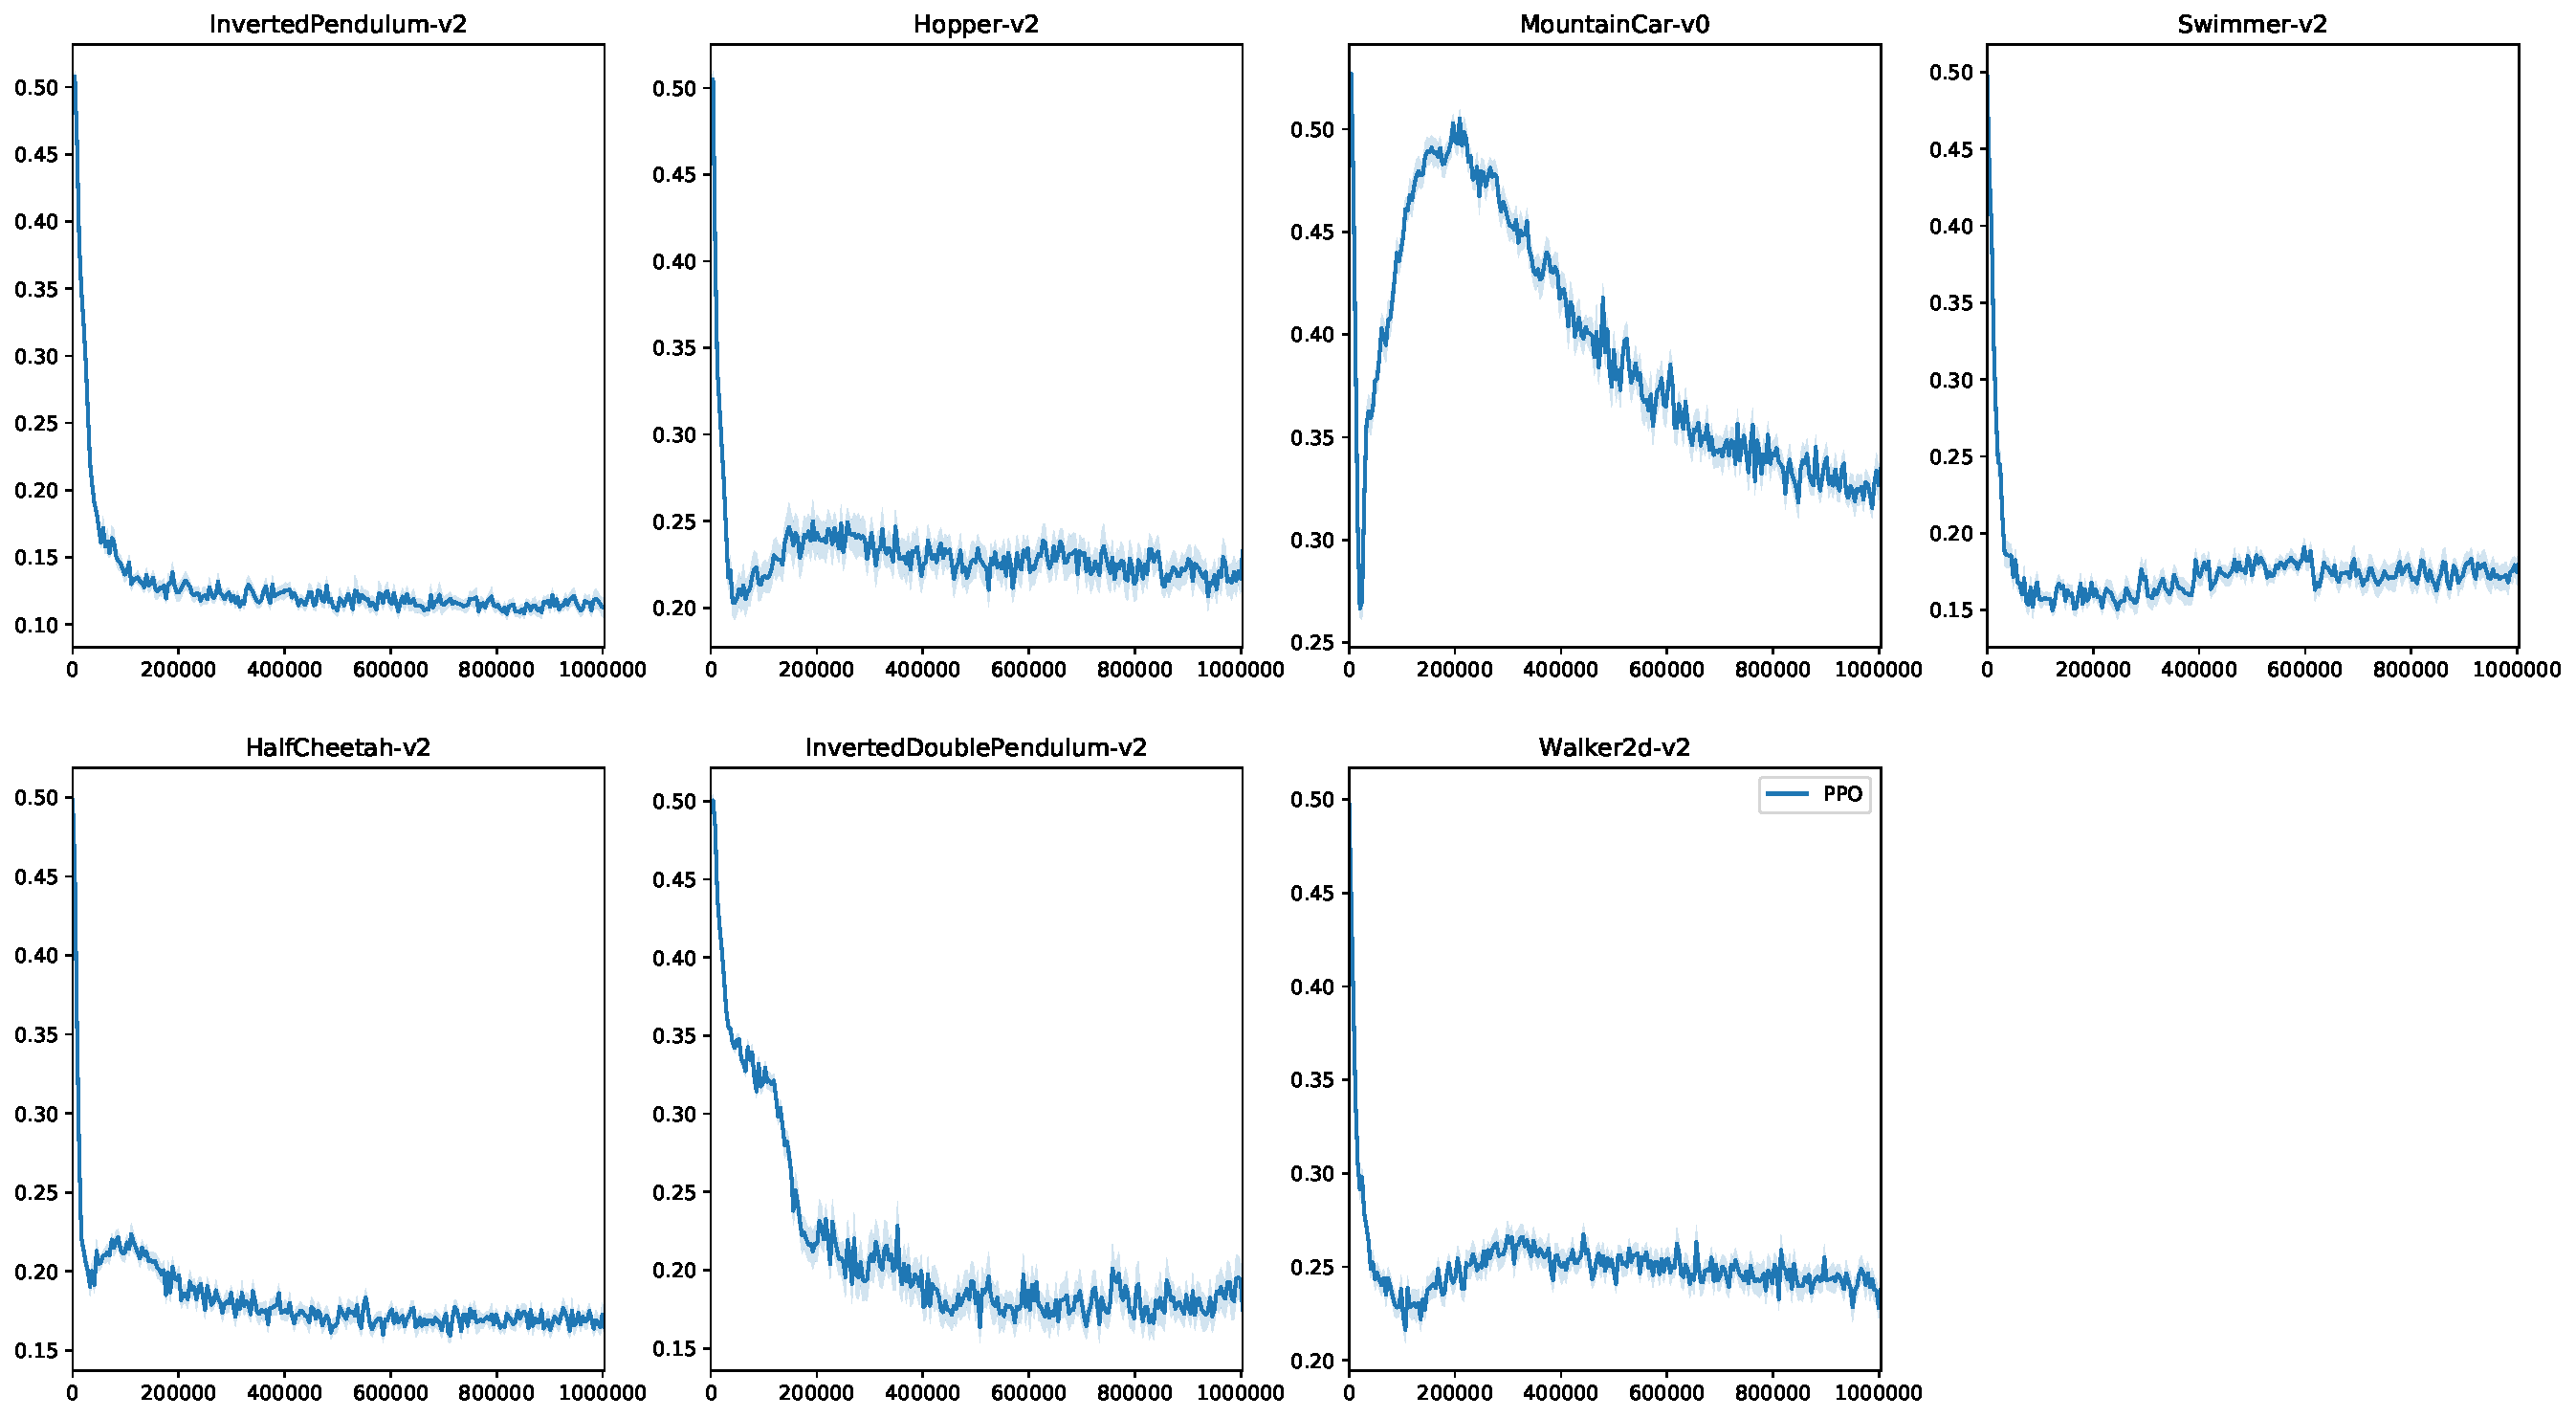
\includegraphics[scale=0.34]{fig/beta_mean.pdf}
    \caption{Mean beta values using recurrent PPO on Mujoco domains}
    \label{fig:beta_mean}
\end{figure}\begin{figure}
    \centering
    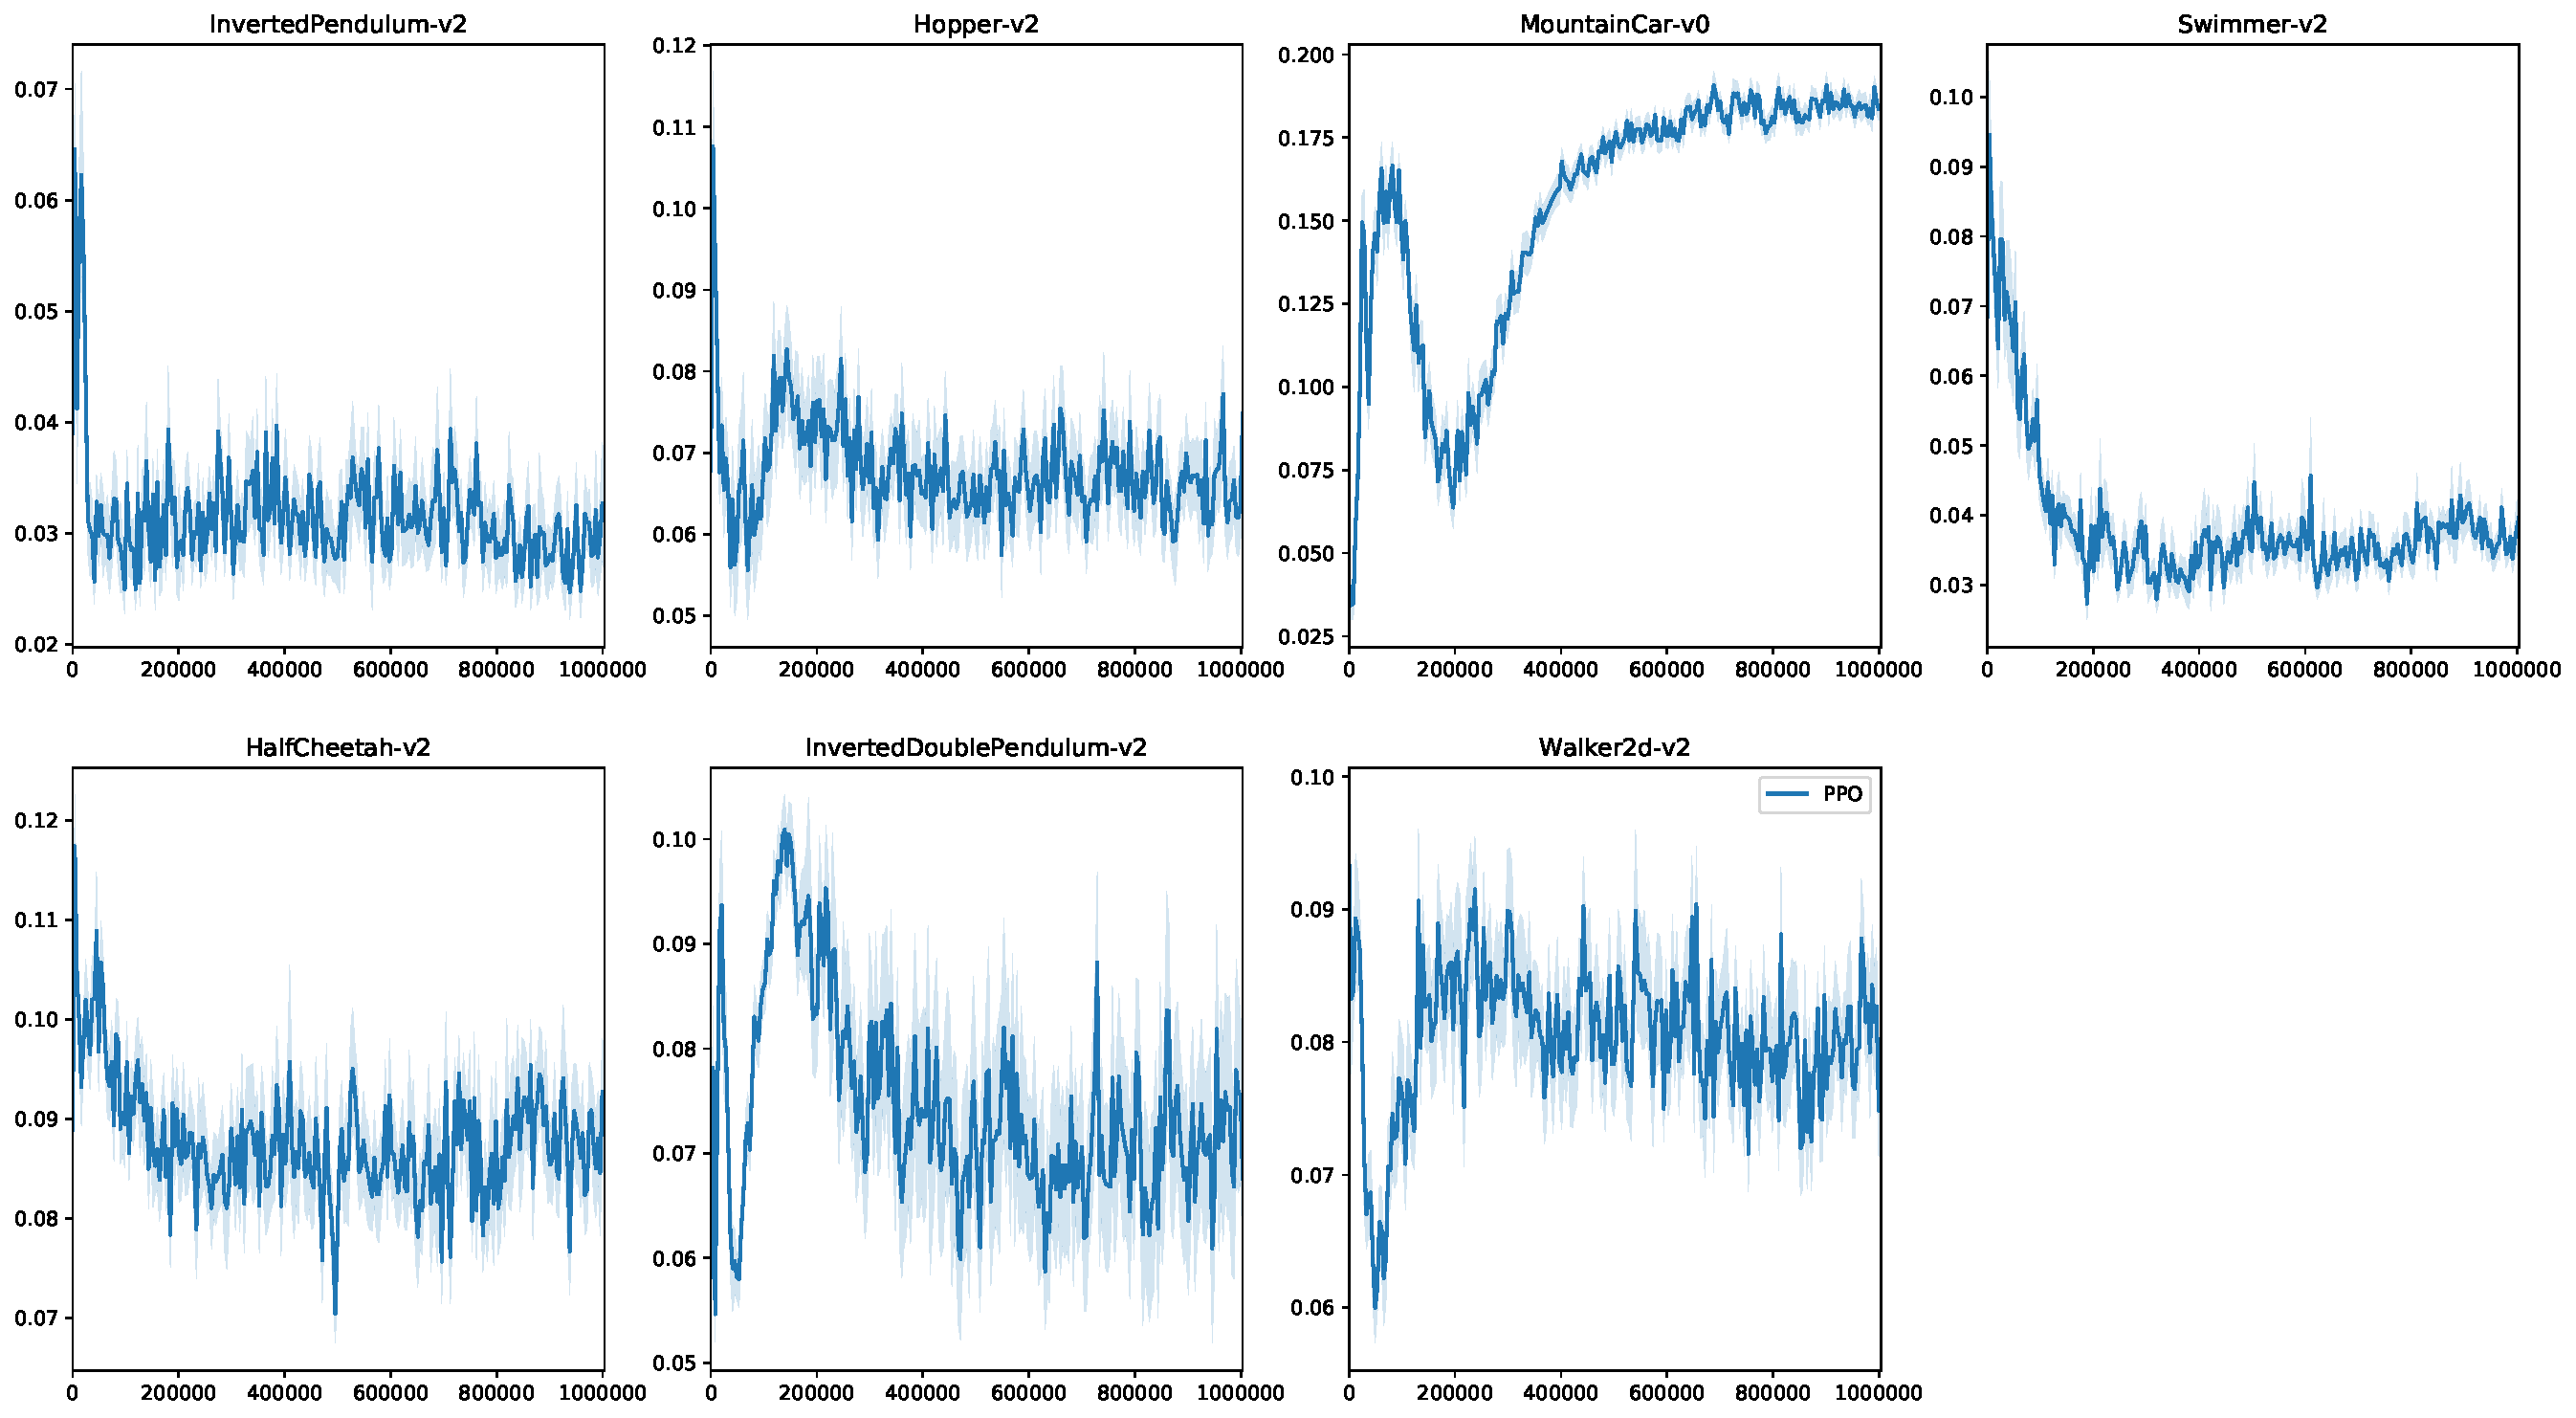
\includegraphics[scale=0.34]{fig/beta_std.pdf}
    \caption{Standard variation of beta using recurrent PPO on Mujoco domains}
    \label{fig:beta_std}
\end{figure}
The algorithm was tested on seven different games of the Mujoco suite (\cite{todorov2012mujoco}). As demonstrated in the figure \ref{fig:perf_mujoco}, we observe an increase in performance on four of the tasks (Swimmer, Hopper, Inverted Pendulum, Double Inverted Pendulum). The performances are averaged over 20 seeds and a confidence interval of $95\%$ is used. For the other three tasks (Half Cheetah, Walker, Mountain Car) the performances were found to be comparable. The performance graphs for all the games can be found in figure \ref{fig:full_mujoco} in the appendix. The mean beta values and variance for all the tasks can also be found in the appendix (figure \ref{fig:beta_mean},\ref{fig:beta_std}).
One interesting finding in the figure \ref{fig:perf_mujoco} concerns inverted-pendulum in the context of generalization. Though the convergence is quick for PPO, severe performance drops (reward drop by more than $100$) can be observed. We found that recurrent learning stabilizes the learning and suffer significantly less drops during training. We notice that on an average PPO will suffer from 5.91 drops below 900 points over 500k steps. In contrast, recurrent learning will only drop 3.53 times. This represent a 40\% drop in \emph{catastrophic forgetting} underlying the potential robustness of recurrent learning.

\subsubsection{Qualitative interpretation of $\param$ }
\begin{figure*}[h]
    \centering
    \begin{minipage}[b]{0.18\linewidth}
    \centering
    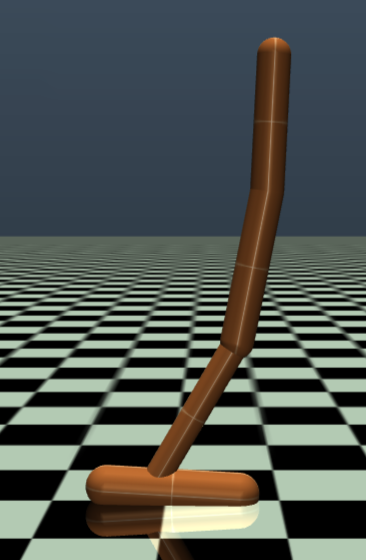
\includegraphics[width=\textwidth,height=2.8cm]{fig/phase_0.png}
    Phase 1: high $\param$
    \label{fig:phase_0}
    \end{minipage}
    \hspace{0.02cm}
    \begin{minipage}[b]{0.18\linewidth}
    \centering
    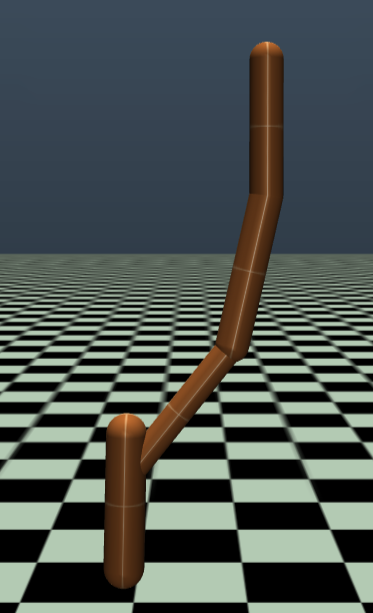
\includegraphics[width=\textwidth,height=2.8cm]{fig/phase_1.png}
    Phase 2: low $\param$
    \label{fig:phase_1}
    \end{minipage}
    \hspace{0.02cm}
    \begin{minipage}[b]{0.18\linewidth}
    \centering
    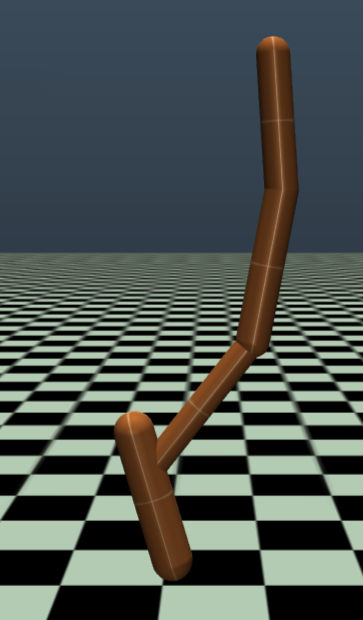
\includegraphics[width=\textwidth,height=2.8cm]{fig/phase_2.png}
    Phase 3: high $\param$
    \label{fig:phase_2}
    \end{minipage}
    \hspace{0.02cm}
    \begin{minipage}[b]{0.18\linewidth}
    \centering
    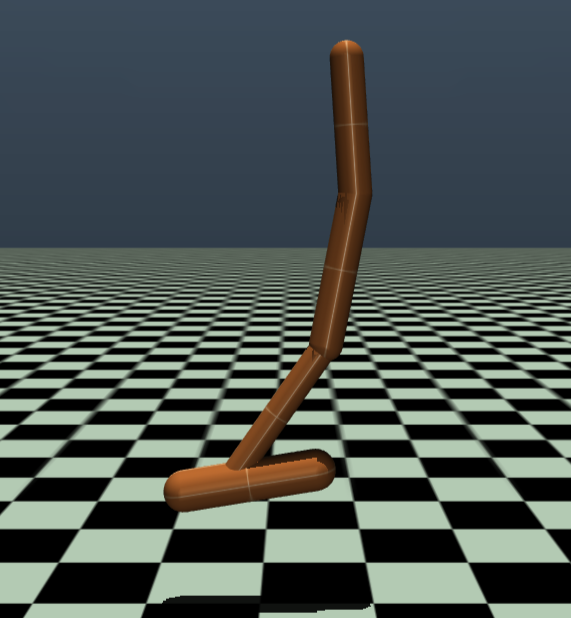
\includegraphics[width=\textwidth,height=2.8cm]{fig/phase_3.png}
     Phase 4: low $\param$
    \label{fig:phase_3}
    \end{minipage}
    \hspace{0.02cm}
    \begin{minipage}[b]{0.18\linewidth}
    \centering
    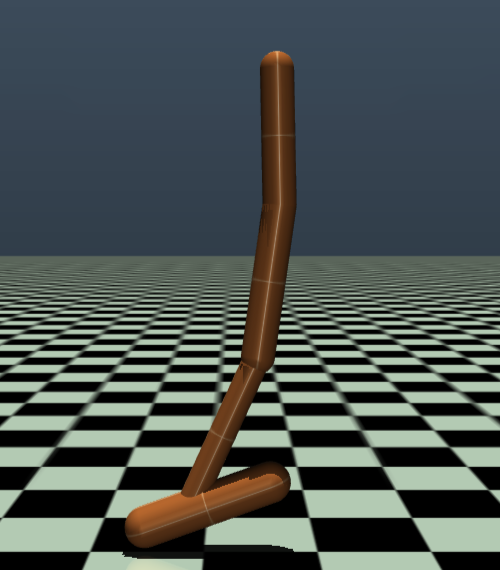
\includegraphics[width=\textwidth,height=2.8cm]{fig/phase_4.png}
    Phase 1: high $\param$
    \label{fig:phase_4}
    \end{minipage}
    \caption{Visual illustration of the cyclical behavior of $\param$ on Hopper}
    \label{fig:visual_hopper}
\end{figure*}


\begin{figure}[!h]
    \centering
    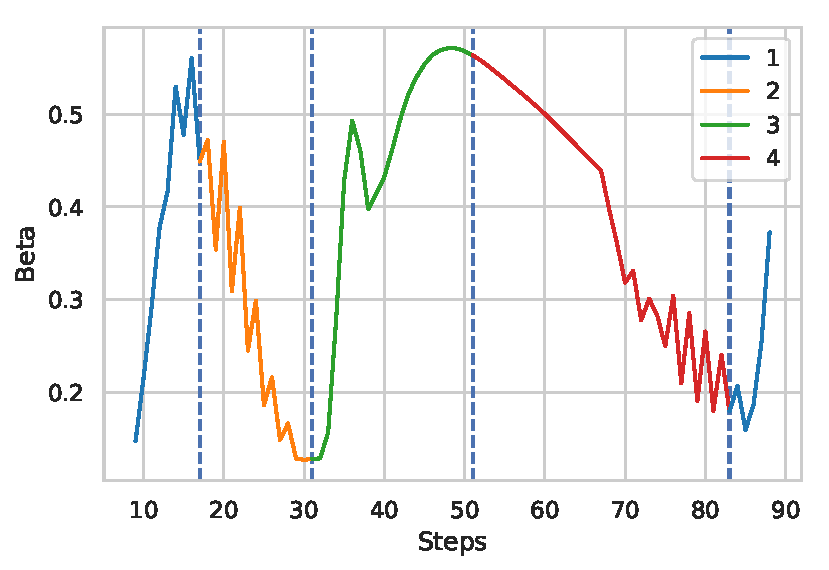
\includegraphics[scale=0.5]{fig/beta_hopper.pdf}
    \caption{Behavior of $\param$ through the trajectory on Hopper with the different phase described in figure $6$-$10$.}
    \label{fig:cyle_hopper}
\end{figure}

\emph{Hopper}: At the end of training, we qualitatively analyze $\param$ through the trajectory and observe the cyclical behavior shown in figure \ref{fig:cyle_hopper}, where different colors describe various stages of the cycle. One intuitive way to look at $\param$ is: \emph{if I were to give a different value to a state would that alter my policy significantly?} We observe an increase in $\param$ value when the agent has to take an important decision like jumping or landing. We see a decrease in $\param$ when the agent has trivial actions to perform. This pattern is illustrated in the figure \ref{fig:visual_hopper} and \ref{fig:cyle_hopper}. This behaviour is cyclic and repetitive and a video of the same can be found at the following link\footnote{\url{https://youtu.be/0bzEcrxNwRw}{}}. One surprising fact was that this behavior was obtained without any regularization on $\param$. Similar behavior can be observed with regularization although the mean and variance of $\param$ diminishes.\\
 \begin{figure}
     \centering
     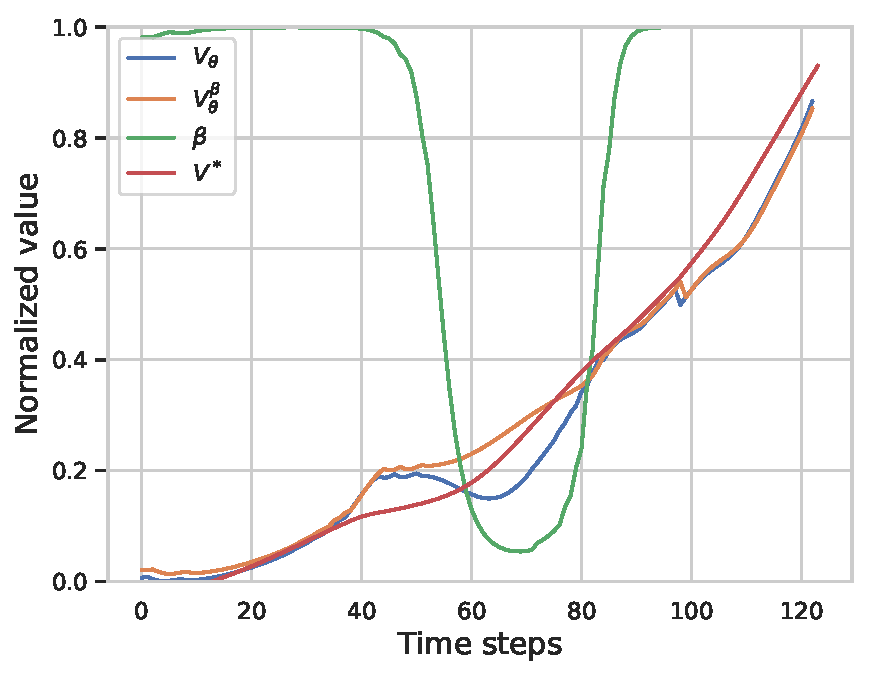
\includegraphics[scale=0.45]{fig/mountain.pdf}
     \caption{Behavior of $\param$ and the value function on Mountain-Car}
     \label{fig:my_label}\label{mountain_car}
 \end{figure}
\emph{Mountain car}: Two scenarios may happen when the agent is climbing up the hill on the right side. Either the agent has enough velocity to finish the game and obtain a high reward, or it doesn't have enough velocity and goes back down the hill. During early stages of training, the function approximator is confused about the scenarios mentioned earlier, resulting a drop in value function around step 100 as shown in figure \ref{mountain_car}. The value increases again once the agent climbs the hill with more velocity. In PPO, we can obtain a more accurate target by setting $\tau$ to a high value, thereby eliminating a drop in value. This enables the $\param$ network to learn to trust its past estimate rather than the noisy point estimate, hence a significant drop in the $\param$ value. As a result, $\vr$ becomes a  better estimate of the target than $\Vt$ in this scenario. After training PPO for a while this drop disappears and the $\param$ mean goes to 1. This experiment shows the potential of $\param$ to smooth out noisy estimates in the trajectory. One caveat to consider is the feedback loop induced by ignoring a state in control. When the policy changes a state that can be ignored at the beginning may be essential later on. One way to address this is to avoid saturating $\param$ such that learning remains possible later on.


\section{Discussions}
\subsection{$\param$ as an interest function:} One interesting result of this work is that the $\param$ network learns to ignore some state without any restrictions imposed on it. It does so in order to reduce the variance. Furthermore, this $\param$ can be interpreted as an \emph{interest} function. In reinforcement learning, having access to a function quantifying the \emph{interest} (\cite{mahmood2015emphatic}) of a state can be helpful. For example, one could decide to explore from those states, prioritize experience replay based on those states. Further work can be done to study how $\param$ may impact performance. We also believe $\param$ can be related to the concepts of bottleneck state (\cite{tishby2011information}). Finally, the concept of interest state in recurrent learning aligns well with the notion of interest state for the $\lambda$ return. Indeed bootstrapping on states with similar values than the one estimated will only result in variance. The most informative updates comes from bootstrapping on state with different value. 

\subsection{Partial observability:} As demonstrated in the experiments earlier, recurrent learning is able in some cases to correctly estimate the value of aliased state using trajectory's estimate. This is a promising area to research as the experiments suggest that ignoring an uninformative state can sometimes be enough to learn its value function. This is in contrast to traditional POMDP method that attempts to infer the belief state. Inferring the true underlying state is not always feasible. In some cases learning to ignore aliased state and relying on previous estimates may be an easier task.
\subsection{Relationship between $\lambda$ and $\param$:} There exists an important relationship between $\lambda$ and $\param$. $\param$ can choose to ignore a state if the past is different from the future. We could get a better estimate of the future using $\lambda$ returns when compared against one step methods. Hence, a need for long horizon to learn accurate $\param$. This behaviour can also be seen in our \emph{mountain car} experiment. Also, bootstrapping from states that are ignored would be detrimental to the learning process. A state is never updated if it has $\param=0$ hence bootstrapping from this state will induce \emph{wrong} bias. To avoid this issue, one approach could be to use learned $\param$ as a state dependent $\lambda$ hence making correct updates.
\subsection{Asymptotic convergence:} As mentioned previously assumption 2 is too restrictive to guarantee convergence in all tabular settings. This analysis could be refined by considering the trajectory's information to bound $\Delta$. As an example, one could consider any physical system where transition in the state space are smooth (continuous state space) and bounded by some Lipschitz constant in a similar manner than (\cite{shah2018q}). 
\subsection{Bias of the eligibility trace:}
We showed in Eq. \eqref{trace} a technique to compute the gradient of the estimate recursively. This technique is computationally inexpensive compared to the recursive backpropogation as the gradient from the past is accumulated. But this kind of an update is biased. This bias comes from the fact that the true gradient obtained by applying the chain rule at future step is different than the trace if the parameters are updated at each time step. This is a similar problem encountered by eligibility traces (\cite{seijen2014true}) and real time recurrent learning (\cite{williams1995gradient}). Similar idea than (\cite{seijen2014true}) may be used to obtain an unbiased estimate.
\subsection{Recurrent learning for action:} We have not explored the concept of recurrent learning for actions (Q values and policy gradient). This is a promising area as constraining actions to be temporally coherent is a natural prior to induce on a function approximator. This technique could also be interesting in the context of exploration as this could yield a \emph{structured exploration}. Finally, this framework with learning $\param$ can be cast as a \emph{vanilla} version of options (\cite{sutton1999between}). 


\paragraph{Conclusion:}





 



%%%%%%%%%%%%%%%%%%%%%%%%%%%%%%%%%%%%%%%%%%%%%%%%%%%%%
% Conclusion
%%%%%%%%%%%%%%%%%%%%%%%%%%%%%%%%%%%%%%%%%%%%%%%%%%%%%
\chapter{Conclusion}
This paper tackles the problem of regularization in RL from a new angle, that is from a temporal perspective. In contrast with typical spatial regularization, where one assumes that rewards are close for nearby states in the state space, temporal regularization rather assumes that rewards are close for states \emph{visited closely in time}. This approach allows information to propagate faster into states that are hard to reach, which could prove useful for exploration. The robustness of the proposed approach to noisy state representations and its interesting properties should motivate further work to explore novel ways of exploiting temporal information.

%%%%%%%%%%%%%%%%%%%%%%%%%%%%%%%%%%%%%%%%%%%%%%%%%%%%%
% Bibliography
%%%%%%%%%%%%%%%%%%%%%%%%%%%%%%%%%%%%%%%%%%%%%%%%%%%%%
%\bibliography{library}
%\bibliographystyle{plain}
\printbibliography
\end{document}